\chapter{COMMUNITY DETECTION IN COMPLEX NETWORKS}
\label{chap:2}
\let\thefootnote\relax\footnotetext{
Portions of this chapter previously appeared as:}
\let\thefootnote\relax\footnotetext{
X. Lu, K. Kuzmin, M. Chen, and B.~K. Szymanski, ``Adaptive modularity maximization via edge weighting scheme,'' {\em Information Sciences}, 2018.\\
}
\let\thefootnote\relax\footnotetext{
Portions of this chapter are submitted as:}
\let\thefootnote\relax\footnotetext{
X. Lu, and B.~K. Szymanski, ``Asymptotic resolution bounds of generalized modularity and statistically significant community detection,'' submitted for publication.}
\let\thefootnote\relax\footnotetext{
X. Lu, and B.~K. Szymanski, ``Regularized Stochastic Block Model for robust community detection in complex networks,'' submitted for publication.}

%%% INTRODUCTION
\section{Introduction}

The study of complex networks reveals the universal principles underlying the network topology. One of the most significant features of complex networks is the community structure, which is widely observed in the social, biological and technological networks. Detecting such community structures can be viewed as partitioning of the network into sub-modules in which the nodes are more densely connected to each other than to the nodes in the rest of the network. Many important tasks, such as data extraction, link prediction, network evolution analysis, and graph mining are based on the community structures discovered in these networks. Therefore, community detection finds its application in a wide variety of research fields, ranging from neurobiology to statistical physics.

Modularity~\cite{newman2006modularity} is perhaps the most widely used quality metric for network partitions. It measures the difference between the observed fraction of edges within a community and this fraction expected in a random graph with the same number of nodes and the same degree sequence. Due to the implicit dependence of modularity definition on a constant (explicitly defined in the generalized modularity as a resolution parameter), however, modularity maximization suffers from the resolution limit problem~\cite{fortunato2007resolution,lancichinetti2011limits} which causes the small, well-formed communities to be merged into a large community since this merging increases modularity. In Section~\ref{sec:2.1}, we review the definition of modularity and its generalized version and weighted version, followed by the discussion of the resolution limit of modularity maximization.

Besides modularity maximization approaches, an alternative method to detect communities is to use the statistical inference to fit a generative random graph model to the observed network data. The maximization of generalized modularity is shown to be equivalent to the maximum likelihood estimation of the degree-corrected planted partition model on the same graph when the resolution parameter takes a particular value~\cite{newman2016equivalence}. Such equivalence shows that modularity maximization is a special case of the statistical inference of random graph models. Modularity maximization assumes all the communities in the network are similar – which is the major cause for the resolution limit problem as we will see in Section~\ref{sec:2.3}. Section~\ref{sec:2.2.2} reviews the definitions of the stochastic block model, its degree-corrected variant and the planted partition model.

Based on the random graph properties, we establish the asymptotic upper and lower bounds for the resolution parameter of the generalized modularity for the modularity maximization algorithm to recover community structure correctly
~\cite{lu2019asymptotic}. To the best of our knowledge, this is the first result connecting the well-known resolution limit of modularity with the random graph theories. Given a resolution parameter within the established range, we show that the communities with different densities can still be detected by maximizing the generalized modularity, regardless whether the equivalence between generalized modularity maximization and the maximum likelihood estimation of the stochastic block model holds or not. When the resolution parameter of the generalized modularity is larger than the upper bound we developed, some well-formed communities are likely to be spread among multiple clusters to increase the generalized modularity; but when the resolution parameter of generalized modularity is smaller than the lower bound we developed, some communities are inappropriately merged into one large cluster. In Section~\ref{sec:2.3}, we present these theoretical results in details.

Our findings shed light how to adapt the generalized modularity to networks in which there is no universal resolution parameter to detect all communities. Resolution limits of the generalized modularity arise when there are the non-overlapping lower and upper bounds of the resolution parameter in the different subgraphs of the networks. Therefore, either some large well-formed communities are split into multiple clusters or some well-formed communities are inappropriately merged into one large cluster. The issue is analogous to identifying mountains that are located at different plateaus; using a single altitude either would miss the lower mountains, or would treat the higher peaks as one mountain. 

To address the problem mentioned above, in Section~\ref{sec:2.4}, we propose a progressive agglomerative heuristic algorithm that systematically increases the resolution parameter. The algorithm recursively splits the clusters found by the previous branch of recursion to detect smaller communities. As the recursion proceeds, the algorithm gradually increases the resolution parameter for high-resolution community detection in local subgraphs of the network. The algorithm proceeds until the found partition is not statistically significant. Compared with the algorithm using a uniform resolution parameter, our approach avoids getting trapped by the resolution limit and does not require multiple re-estimation of the resolution parameter~\cite{newman2016equivalence} which can be computationally prohibitively costly for large networks.

As we discussed above, given an input network, modularity maximization is one special case of the statistical inference of the degree-corrected stochastic block model. The degree-corrected stochastic block model is able to generate a wide range of structures, ranging from the traditional assortative community structure to the disassortative structures such as the core-periphery and bi-partite networks. The model itself does not impose any constraint on which structure is returned. Instead, the inference algorithm returns the most likely partition of the network according to the maximum likelihood estimations. Thus, the inference algorithms, such as Markov chain Monte Carlo, are likely to get trapped by the local optima of the log-likelihood, corresponding to either assortative or disassortative structures. We propose a regularized model which uses one single model parameter to control the resulting structure assortativity by inference. This regularized model is presented in Section~\ref{sec:2.5}.

In Section~\ref{sec:2.6}, we propose an efficient edge weight scheme to improve the quality of the communities discovered by the state-of-art community detection algorithms~\cite{lu2018adaptive}. The edge weighting scheme samples a small set of connected ground truth communities from a synthetic network sharing similar properties as the input network’s. The changes of modularity upon merging these sampled communities are used as the penalty terms of a regression model which converts the local edge features to the corresponding edge weights. Hence, instead of assigning the edge weights in an ad-hoc style, our proposed edge weighting scheme searches for the most appropriate edge weights automatically. Although the proposed edge weight scheme is based on the modularity maximization only, the edges weights produced by our model also significantly improve many other state-of-the-art community detection algorithms. Section~\ref{sec:2.6} presents the edge weighting scheme and the experimental results on real and synthetic networks.

\section{Related work} \label{sec:2.1}
\subsection{Modularity and resolution limit} \label{sec:2.1.1}
Modularity maximization is one of the state-of-the-art methods for community detection that has gained popularity in the last decade. The goal of the modularity maximization is to discover community structure in a network by maximizing the modularity, defined as
\begin{equation} \label{eq:definition}
    Q = \frac{1}{2m} \sum_{r} \sum_{\{i,j\}\in r} \left( A_{ij} - \frac{ k_i k_j }{ 2m } \right),
\end{equation}
where $A_{ij}$ is the number of edges between nodes $i$ and $j$ and $\{i,j\} \in r$ denotes all the pairs of nodes $i$ and $j$ in the same block $r$, $k_i$ is the degree of node $i$ and $m$ is the total number of edges in the network. In an unweighted undirected network, $2 m = \sum_i k_i$ because every edge has exact two endpoints by definition.

Modularity can be also written in an alternative way as
\begin{equation} \label{eq:modularity_definition_alternative}
    Q = \sum_{r} \left[\frac{m_r}{m} - \left(\frac{\kappa_r}{ 2m } \right)^2 \right],
\end{equation}
where $m_r$ is the number of edges with both endpoints inside the community $r$, $\kappa_r = \sum_{i \in r} k_i$ is the sum of the degrees of nodes in community $r$, and $m$ is the total number of edges in the network.

The generalized modularity of Reichardt and Bornholdt~\cite{reichardt2006statistical} incorporates a simple resolution parameter $\gamma$ and is defined as a function of $\gamma$ as follows:
\begin{equation} \label{eq:modularity_definition}
    Q(\gamma) = \frac{1}{2m} \sum_{r} \sum_{\{i,j\}\in r} \left( A_{ij} - \gamma \frac{ k_i k_j }{ 2m } \right).
\end{equation}
The definition of the generalized modularity does not provide the value of the resolution parameter. The alternative of the generalized modularity is
\begin{equation} \label{eq:g_modularity_definition_alternative}
    Q(\gamma) = \sum_{r} \left[\frac{m_r}{m} - \gamma \left(\frac{ \kappa_r }{ 2m } \right)^2 \right],
\end{equation}

The modularity can be naturally extended to the networks with weighted edges by replacing the count of edges with the sum of their weights. Hence, the weighted modularity is defined as
\begin{equation} \label{eq:weighted_modularity_definition}
    Q(\gamma) = \frac{1}{2W} \sum_{r} \sum_{\{i,j\}\in r} \left( W_{ij} - \gamma \frac{ w_i w_j }{ 2W } \right),
\end{equation}
where $W$ is the sum of weights of edges in the entire graph, $W_{i,j}$ is the weight of the edge between nodes $i$ and $j$, $w_i$ is the sum of the weights of edges adjacent to node $i$. The original definition of modularity is a special case of the weighted version when the weight of every edge is 1.

For the modularity maximization to be able to find a community $r$ with $m_r$ edges inside, the following inequality must hold~\cite{fortunato2007resolution},
\begin{equation}
m_r \geq \sqrt{\frac{m}{2}}.
\end{equation}
where $m_r $ is the number of the edges inside community $r$, and $m$ is the total number of edges of the entire graph. In large networks with millions of edges, the number of edges in most communities is often smaller than this lower bound. In such cases, the small, well-formed communities are often merged into a large cluster to increase the modularity. This problem is also referred to as the resolution limit of modularity.

\subsection{Stochastic Block Model} \label{sec:2.2.2}
The standard stochastic block model is a generative model of the graph in which nodes are organized as blocks and edges are placed between nodes independently at random, with a probability determined by the block assignments of the endpoints. Hence, the nodes in the same block are statistically indistinguishable from each other by definition. The standard stochastic block model assumes the number of edges between nodes $i$ and $j$ is independently distributed Bernoulli with mean $\omega_{g_i,g_j}$, where for any node $l$, $g_l$ denotes the block assignment of node $l$. The stochastic block model is fully specified by the block assignment $g_i$ for each node $i$ and the edge probability $\omega_{rs}$ for all pairs of blocks $(r,s)$. Since the standard stochastic block model considers nodes in the same block statistically indistinguishable, the most likely block assignment often groups the nodes of similar degrees in a block, resulting in lower and higher-degree blocks, rather than the traditional community structures. Reference \cite{karrer2011stochastic} extends the standard stochastic block model by incorporating the node degrees. This simple yet effective modification improves the performance of the models for statistical inference of group structure in the real-world networks, by allowing nodes in a community to have broad range of degrees. To simplify technical derivations, authors in \cite{karrer2011stochastic} replace the Bernoulli distribution by the Poisson one. Compared to many community detection algorithms proposed in an ad-hoc manner, the statistical inference from stochastic block model is a more systematic approach which discovers modular structures with theoretical guarantees~\cite{bickel2009nonparametric}; thus, it has gained significant attention in recent years.

Formally, let $\bf A$ be the adjacency matrix whose component $A_{ij}$ denotes the number of edges between nodes $i$ and $j$ in an unweighted undirected multigraph. In a network with self-loop edges (edges connecting a node to itself), a node $i$ with $k$ self-loop edges is represented by the diagonal adjacency matrix element $A_{ii} = 2k$. Multi-edges and self-loop edges are practical in certain networks such as the web network where a web page may contain multiple hyperlinks pointing to other pages and to itself. Such edges are less common in social networks. However, most social networks are very sparse, so the impact of multi-graphs and self-loop edges can be neglected.

Suppose the number of edges between two different nodes $i$ and $j$ follows the Poisson distribution with mean $\eta_{ij}$ and the number of self-loop edges at node $l$ follows the Poisson distribution with mean $\frac{1}{2}\eta_{ll}$. The likelihood of generating $\bf A$ is
\begin{equation} \label{eq:ll0}
    \log P({\bf A}|\{\eta_{ij}\}) = \prod_{i} \frac{(\frac{1}{2}\eta_{ii})^{A_{ii}/2} }{(\frac{1}{2}A_{ii})!} e^{-\eta_{ii}/2} \prod_{i<j} \frac{\eta_{ij}^{A_{ij}} }{A_{ij}!} e^{- \eta_{ij}}.
\end{equation}
Note that $\eta_{ij}$ is defined as the number of edges here and not, as customary, the probability because multi-edges are allowed in our model.

In an unweighted undirect network, after ignoring all terms independent of the $\eta_{ij}$s, the log-likelihood above simplifies to
\begin{equation} \label{eq:ll}
    \log P({\bf A}|\{\eta_{ij}\}) = \frac{1}{2} \sum_{ij} \Big(A_{ij} \log \eta_{ij} - \eta_{ij} \Big).
\end{equation}

The degree-corrected stochastic block model~\cite{karrer2011stochastic} assumes $\eta_{ij} = \omega_{g_i,g_j} \theta_i \theta_j$ where for any  node $l$, $\theta_l$ is a parameter associated with this node and $g_l$ is its block assignment. Given a partition of the network, i.e. its block assignments $\{g_i\}$, the posterior maximum likelihood estimates of $\theta_i$ and $\omega_{rs}$ are 
\begin{equation}
    \hat{\theta}_i = \frac{k_i}{\kappa_{g_i}}, \quad \quad \hat{\omega}_{rs} = m_{rs},
\end{equation}
where $k_i$ is the degree of node $i$, $\kappa_{r}$ is the sum of the degrees of all nodes in a block $r$, and $m_{rs}$ is the total number of edges between blocks $r$ and $s$, or twice the number of edges in $r$ if $r=s$. Formally,
\begin{equation} \label{eq:number_edges}
    \kappa_r = \sum_{i\in r} k_i, \quad \quad m_{rs} = \sum_{i\in r} \sum_{j\in s} A_{ij},
\end{equation}
where $i\in r$ denotes all nodes in the blocks $r$. For simplicity, we define $m_c$ as the number of edges with both endpoints in community $c$, so $m_{cc} = 2m_c$, and $m$ is defined as the total number of edges in the entire network.

Given the MLEs of $\theta_k$ and $\omega_{g_i g_j}$, the expected number of edges between nodes $i$ and $j$ can be written as
\begin{equation} \label{eq:mle_dsbm}
    \eta_{ij} = m_{g_i g_j} \frac{k_i}{\kappa_{g_i}} \frac{k_j}{\kappa_{g_j}}.
\end{equation}
Therefore, maximizing the log-likelihood in Eq.~\ref{eq:ll} is equivalent to maximizing
\begin{equation}
    \log P({\bf A}|\{\eta_{ij}\}) = \sum_{rs} m_{rs} \log \frac{m_{rs}}{\kappa_{r}\kappa_{s}}.
\end{equation}
This criterion turns to have an information-theoretic interpretation when it is presented in the alternative form 
\begin{equation} \label{eq:KL_divergence}
     \log P({\bf A}|\{\eta_{ij}\}) = \sum_{rs} \frac{m_{rs}}{2m} \log \frac{ \frac{m_{rs}}{2m} }{\frac{\kappa_{r}}{2m} \frac{\kappa_{s}}{2m}},
\end{equation}
which is equal to the Kullback-Leibler divergence~\cite{kullback1951information} between the probability of observing an edge $(i, j)$ pointing from block $r$ toward $s$, i.e. $P[i\in r, j\in s] = m_{rs}/{2m}$, and the corresponding probability in a random graph with the same degree sequence, i.e. $P' [i\in r, j\in s] = (\kappa_{r}/2m)(\kappa_{s}/{2m})$.

The degree-corrected planted partition model~\cite{newman2016equivalence} is a special case of the degree-corrected stochastic block model in which the expected number of edges $\eta_{ij}$ in a graph has the form
\begin{equation} \label{eq:pp_form}
\eta_{ij} = 
    \begin{cases}
         \omega_{1} \theta_i \theta_j    & \text{if  } g_i = g_j,  \\
         \omega_{0} \theta_i \theta_j  & \text{otherwise}. \\
    \end{cases}
\end{equation}
Hence, the degree-corrected stochastic block model reduces to the degree-corrected planted partition model when the parameters $\omega_{rr} = \omega_1$ for all $r$ and $\omega_{rs} = \omega_0$ for all pairs $r,s$ such that $r\neq s$.

Newman~\cite{newman2016equivalence} shows the maximization of the generalized modularity is equivalent to the maximum-likelihood estimation (MLE) of the degree-corrected planted partition model~\cite{karrer2011stochastic} on the same graph. In other words, the partition of the network which best fits the degree-corrected planted partition model to the network data also maximize the generalized modularity given the corresponding resolution parameter.

The degree-corrected stochastic block model~\cite{karrer2011stochastic,newman2016equivalence} incorporates the heterogeneous node degrees in the real networks. Reference~\cite{newman2016equivalence} assumes the number of edges between nodes $i$ and $j$ follows the Poisson distribution with mean $\eta_{ij} = \omega_{g_i,g_j} \frac{k_i k_j}{2m}$ where $m$ is the total number of edges in the network. The denominator $2m$ is only optional, but it is convenient for technical derivation as shown below. This definition is actually equivalent to the definition in Eq.~\ref{eq:mle_dsbm} but the parameter $\omega_{rs}$ here has a different meaning. To distinguish this definition from the original definition of expected number of edges in~\cite{karrer2011stochastic}, in the rest of this paper, we call $\omega_{rs}$ the \textit{{\bf \it density}} of the edges between blocks $r,s$. When $r=s$, $\omega_{rs}$ corresponds to the intra-community edge {\it density}; otherwise, $\omega_{rs}$ is called the inter-community edge {\it density}. Accordingly, the $(r, s)$-th element of the {\it density} matrix $\Omega$ is $\omega_{rs}$. Besides, we assume that a group of nodes in the same block of the stochastic block model represents a single community. Following this line of reasoning, the degree-corrected planted partition model~\cite{newman2016equivalence} defines the expected number of edges between two nodes, $i$ and $j$, as   
\begin{equation} \label{eq:pp}
\eta_{ij} = 
    \begin{cases}
         \omega_{1} \frac{k_i k_j}{2m}    & \text{if  } g_i = g_j,  \\
         \omega_{0} \frac{k_i k_j}{2m}  & \text{otherwise}. \\
    \end{cases}
\end{equation}
Hence, the {\it density} matrix $\Omega$ of this degree-corrected planted partition model only involves two possible values, i.e., $\Omega=\{\omega_{1}, \omega_{0}\}$.

Substituting Eq.~\ref{eq:pp} into Eq.~\ref{eq:ll}, the log-likelihood for the degree-corrected planted partition model, after a small amount of manipulation, becomes 
\begin{equation} \label{eq:modularity}
    \log P({\bf A}|\Omega, {\bf g}) = B \left[ \frac{1}{2m} \sum_{r} \sum_{\{i,j\} \in r} \left(A_{ij} - \gamma \frac{ k_i k_j }{ 2m } \right) \right] + C + D,
\end{equation}
where $\{i,j\} \in r$ denotes all the pairs of nodes $i$ and $j$ in the same block $r$, $B$ and $C$ are constants that depend on $\Omega=\{w_1,w_0\}$ but not on the block assignment ${\bf g} = \{g_i\}$, specifically,
\begin{equation} \label{eq:BCD}
    \begin{split}
        B&= m \left(\log \omega_1 - \log \omega_0 \right) \\
        C&= m \left(\log \omega_0 - \omega_0 \right) \\
        D&= \sum_i k_i \log k_i - \log \left(2m \right)
    \end{split}
\end{equation}
and the resolution parameter $\gamma$ in Eq.~\ref{eq:modularity} is a resolution parameter defined as
\begin{equation}~\label{eq:gamma_mle}
    \gamma = \frac{\omega_{\text{1}} - \omega_{\text{0}}}{\log \omega_{\text{1}} - \log \omega_{\text{0}}}.
\end{equation}
Note that the log-likelihood here is exact for undirected unweighted multigraphs; it has a slightly different form than the derivation in~\cite{newman2016equivalence} where constant term $D$ is ignored as it is independent from the parameters $\Omega$ and $\bf g$. Since $B$, $C$ and $D$ are constants given the value of $\Omega$, the maximum likelihood estimation of $\bf g$ is then equivalent to maximizing the generalized modularity
\begin{equation}
    Q(\gamma) = \frac{1}{2m} \sum_{r} \sum_{\{i,j\}\in r} \left( A_{ij} - \gamma \frac{ k_i k_j }{ 2m } \right).
\end{equation}
Since maximizing the log-likelihood in Eq. \ref{eq:modularity} is equivalent to maximizing the generalized modularity with resolution parameter defined in Eq. \ref{eq:gamma_mle}, it shows an exact equivalence between maximization of the generalized modularity that includes a specific resolution parameter and the degree-corrected planted partition model.

It is worth noting that the resolution parameter $\gamma$ must satisfy Eq.~\ref{eq:gamma_mle} to guarantee the equivalence between the generalized modularity maximization and the maximum likelihood estimation of degree-corrected planted partition model. This is a drawback because the correct value of resolution parameter in Eq.~\ref{eq:gamma_mle} is unknown before we can estimate $\omega_1$ and $\omega_0$. Given a network generated by the degree-corrected planted partition model, however, one needs the ground truth communities to calculate $\omega_1$ and $\omega_0$. That being said, one must make an initial guess of the $\gamma$ value so that the generalized modularity maximization algorithm can detect communities with it. But this initial guess of $\gamma$ may not satisfy Eq.~\ref{eq:gamma_mle}.

Reference \cite{newman2016equivalence} proposes an iterative algorithm to find the optimal value of $\gamma$ which maximizes the log-likelihood of Eq.~\ref{eq:modularity}. It makes an initial guess of the $\gamma$ value to detect communities by maximizing the generalized modularity. Given these detected communities, the $\gamma$ value gets updated by Eq.~\ref{eq:gamma_mle} using the maximum likelihood estimates of $\omega_1$ and $\omega_0$ which are equal to
\begin{equation} \label{eq:update_omega}
    \hat{\omega}_1 =  \frac{2\sum_r m_r}{\sum_r \kappa_r^2 / 2m}, \quad \quad \quad \hat{\omega}_0 = \frac{2m - 2\sum_r m_r}{2m - \sum_r \kappa_r^2 / 2m},
\end{equation}
where $m_r$ is the number of edges with both endpoints in the community $r$, i.e. $m_r = \frac{1}{2}m_{r,r}$ as defined by Eq.~\ref{eq:number_edges} and $\kappa_r$ is the sum of degrees of the nodes in the community $r$. The iterative algorithm repeats the following two steps until the $\gamma$ value becomes stable:
\begin{itemize}
    \item Given the current $\gamma$, find the block assignment which maximizes the generalized modularity $Q(\gamma)$, i.e., ${\bf g}^{\text{new}} = \argmax_{\bf g} Q(\gamma)$.
    \item Given the current block assignment ${\bf g}$, calculate the maximum likelihood estimates of $\omega_1$ and $\omega_0$ using Eq.~\ref{eq:update_omega} and update the $\gamma$ value by Eq.~\ref{eq:gamma_mle} accordingly.
\end{itemize}

\subsection{Metrics comparing network partitions} \label{sec:2.2.3}
The computation of modularity does not require the ground truth labels of the detected communities in a network. When the ground truth communities are available, the following metric are also generally used to evaluate the quality of the detected communities.

Let the ground truth partition of the graph be denoted as $GN=\{g_1, g_2,\ldots\}$ where $g_i$ is the set of nodes in a single ground truth community, and the detected communities be denoted as $C=\{c_1, c_2,\ldots\}$ where $c_i$ is the set of nodes in single community discovered the community detection algorithm. The following evaluation metrics measure the similarity between the produced partition $C$ and ground truth partition $GN$.

\textbf{Variation of Information} (VI)~\cite{good2010performance} measures the similarity between $C$ and $GN$ based on information theory
\begin{equation}
VI(C, GN) = H(C) + H(GN) - 2I(C, GN)
\end{equation}
where $I(C,GN)=H(C) + H(GN) - H(C,GN)$ is the \textit{Mutual Information}, and $H()$ is the entropy function defined as
\begin{align}
H(C) &= -\sum_{c_i \in C} p(c_i) \log{p(c_i)} = -\sum_{c_i \in C} \frac{|c_i|}{|V|} \log{ \frac{|c_i|}{|V|} }\\
H(C,GN) &= -\sum_{c_i \in C, g_i \in {GN}} p(c_i,g_i) \log{p(c_i,g_i)} \nonumber\\
&= -\sum_{c_i \in C, g_i \in {GN}} \frac{|c_i \cap g_i|}{|V|} \log{ \frac{|c_i \cap g_i|}{|V|} }
\end{align}

\textbf{Normalized Mutual Information} (NMI)~\cite{wagner2007comparing} is defined as
\begin{equation} \label{eq:NMI}
NMI(C,GN)= \frac{2I(C,GN)}{H(C) + H(GN)}
\end{equation}

\textbf{Adjusted Mutual Information} (AMI)~\cite{vinh2010information} is defined as
\begin{equation}
AMI(U,Q)= \frac{I(C,GN) - E\left[I(C,GN)\right]}{max\left\{H(C), H(GN)\right\} - E\left[I(C,GN)\right]}
\end{equation}
where $E\left[I(C,GN)\right]$ is the expected mutual information between two random clusterings as defined in \cite{vinh2010information}.

\textbf{F-measure}~\cite{wagner2007comparing} is given as
\begin{equation}
\textit{F-measure}(C,GN) = \frac{1}{|V|}\sum_{c_i \in C} |c_i| \max_{g_i \in GN} \frac{2|c_i \cap g_i|}{|c_i|+|g_i|}
\end{equation}

\textbf{Adjusted Rand Index} (ARI)~\cite{hubert1985comparing} computes the similarity by comparing all pairs of nodes that are assigned to the same or different communities in $C$ and $GN$. Specifically, ARI is defined as
\begin{equation} \label{eq:ARI_definition}
ARI(C,GN) = \frac{  \sum_{ij}{\binom{|c_i \cap g_j|}{2}} - \frac{ [\sum_i {\binom{|c_i|}{2}} \sum_j{ \binom{|g_j|}{2} }   ] } { \binom{|V|}{2} } } {  \frac{1}{2} [\sum_i \binom{|c_i|}{2} + \sum_j \binom{|g_j|}{2} ]  - \frac{ [\sum_i {\binom{|c_i|}{2}} \sum_j{ \binom{|g_j|}{2} }   ] } { \binom{|V|}{2} } }.
\end{equation}

\textbf{Modularity Density}~\cite{chen2014community} is a measure of the quality of communities in a network. Like the original modularity, it does not need the ground truth. The formal definition is
\begin{align}
Q_{ds} &= \sum_{c_i \in C} \left[ \frac{m_{c_i}}{m} d_{c_i} - \left( \frac{\kappa_{c_i}}{2m} d_{c_i} \right)^2 - \sum_{\substack{c_j \in C\\c_j\neq c_i}} \frac{m_{c_i,c_j}}{2m} d_{c_i,c_j}
\right]\\
d_{c_i} &= \frac{2m_{c_i}}{n_{c_i}(n_{c_i}-1)} \quad \quad \quad \quad d_{c_i,c_j} = \frac{m_{c_i,c_j}}{n_{c_i}(n_{c_i}-1)} 
\end{align}
where $n_{c_i}$ is the number of nodes in community $c_i$, $d_{c_i}$ is the internal density of community $c_i$, and $d_{c_i,c_j}$ is the pair-wise density between community $c_i$ and community $c_j$.

\section{Asymptotic resolution bounds of generalized modularity} \label{sec:2.3}
Merging two communities, $r$ and $s$, results in the following equalities: the total number of edges inside the merged community $m_{r\cup s}=m_r+m_s+m_{r,s}$ and the sum of degrees of the nodes inside the merged community $\kappa_{r\cup s} = \kappa_r+\kappa_s$. Hence, given the formalization of the generalized modularity in Eq.~\ref{eq:g_modularity_definition_alternative}, the optimization algorithm is able to detect two well-formed communities $r$ and $s$ if the change of generalized modularity from merging $r$ and $s$ is negative, leading to the inequality
\begin{equation}
\Delta Q(\gamma) = \frac{m_{rs}}{m} - \gamma \frac{\kappa_{r}\kappa_{s}}{2m^2} < 0,
\end{equation}
which can be rewritten in the alternative way as
\begin{equation}\label{eq:resolution_0}
\kappa_{r}\kappa_{s} > 2 \frac{m_{rs} m} {\gamma}.
\end{equation}
Otherwise, when the $\Delta Q(\gamma) \geq 0$, communities $r$ and $s$ are merged to increase $Q(\gamma)$. Clearly, one can always increase $\gamma$ so that Eq.~\ref{eq:resolution_0} holds for any small $\kappa_r$ and $\kappa_s$. But, a large $\gamma$ may result in inappropriate split of some communities. To see this point, consider a community $t$ comprised of two sets of nodes $t'$ and $t''=t-t'$ with sums of degrees $\kappa'$ and $\kappa''$ respectively, and $m''$ edges between nodes in $t'$ and $t''$. To avoid splitting community $t$ into $t'$ and $t''$, the inequality
\begin{equation}~\label{eq:resolution_1}
\kappa'\kappa'' < 2\frac{m''m}{\gamma}
\end{equation}
must hold. Given Eq.~\ref{eq:resolution_0} and Eq.~\ref{eq:resolution_1}, we have
\begin{equation} ~\label{eq:resolution}
  \frac{\kappa'\kappa''}{m''} < \frac{2m}{\gamma} < \frac{\kappa_r \kappa_s}{m_{rs}}.  
\end{equation}
A simple and straightforward explanation of the resolution limit found by Fortunato et al. [11] is that in realistic networks the above inequality may not hold. Indeed, it is likely that in a large network there exist communities $r$ and $s$ with small $\kappa_r$ and $\kappa_s$ and community $t$ with large sum of node degrees $(\kappa'+\kappa'')$, such that the inequality above does not hold because $\frac{\kappa_r \kappa_s}{m_{rs}} < \frac{\kappa'\kappa''}{m''}$, giving rise to resolution limit anomaly.

Newman~\cite{newman2016equivalence} recently has shown that the maximization of generalized modularity on planted partition networks is optimal, because it is equivalent to the maximum-likelihood estimation of the degree-corrected planted partition model as long as the correct resolution parameter is chosen. 

Here we consider the extended planted partition model which allows the {\it density} matrix $\Omega$ to have different values on the diagonal - each community has its own {\it density} $\omega_r$ as the $r$-th element on diagonal of $\Omega$, while keeping the background inter-community {\it density} $\omega_0$, the same as defined in degree-corrected planted partition model in Eq.~\ref{eq:pp}. The definition of the expected number of edges between nodes $i$ and $j$ in this case becomes
\begin{equation} \label{eq:pp_new}
\eta_{ij} = 
    \begin{cases}
        \omega_r \frac{k_i k_j}{2m}  & \text{if  } g_i = g_j = r,  \\
        \omega_0 \frac{k_i k_j}{2m} & \text{if  } g_i \neq g_j. \\
    \end{cases}
\end{equation}

Given the nodes' degrees $k_i$ and $k_j$, $\frac{k_i k_j}{2m}$ is the expected number of edges between nodes $i$ and $j$ in the graph ensembles generated by the configuration model~\cite{molloy1995critical}. Thus, the {\it density} $\omega_r$ can be treated as the relative ratio of the expected number of edges in the extended planted partition model to the corresponding values in configuration model. Given the definition in Eq.~\ref{eq:pp_new}, the corresponding {\it density} matrix of $T$ communities is
\begin{equation} \label{eq:density2}
    \Omega = \text{diag}_T \left(\{\omega_r\} \right) + \left(J_T - I_T\right)\omega_0,
\end{equation}
where $\text{diag}_T(\{\omega_r\})$ represents the diagonal matrix of size $T\times T$ with the intra-community edge {\it densities} $w_1,w_2,\dots,w_T$ on the diagonal, $J_T$ and $I_T$ are correspondingly a matrix with all elements equal to 1 and the identity matrix of size $T\times T$. 

%If $\omega_r>\omega_0$ for each $r$, Eq.~\ref{eq:density2}) %can be rewritten in the alternative form as
%\begin{equation}
%    \Omega = \text{diag}_T(\{\omega_r-\omega_0\}) + J_T %\omega_0.
%\end{equation}
%Hence, the network generated by this model can be treated as %many communities with different {\it densities} embedded in a %random graph where the number of edges between nodes $i$ and %$j$ follows the Poisson distribution with mean $\omega_0 %\frac{k_i k_j}{2m}$. 
The log-likelihood of this extended planted partition model is 
\begin{equation} \label{eq:ll_new}
    \log P({\bf A}|\Omega, {\bf g}) =  \frac{1}{2} \sum_{\{i,j\} \in r} \beta_r \Big(A_{ij} - \gamma_r \frac{k_i k_j}{2m} \Big) + C + D,
\end{equation}
where the expressions of $C$ and $D$ here are the same as mentioned above in Eq.~\ref{eq:BCD}, but the $\gamma$ parameter is replaced by a set of community-specific parameters $\gamma_r$ and the $\beta_r$ defined as
\begin{equation} \label{eq:para}
   \beta_r = \log \omega_r - \log \omega_0, \quad \quad \gamma_r = \frac{\omega_r-\omega_0}{\log \omega_r- \log \omega_0}.
\end{equation}
When all communities has the same edge density $\omega_r$, the log-likelihood of the extended model has the same form as the degree-corrected planted partition model defined by Eq.~\ref{eq:modularity}.

The maximum likelihood estimates of the intra-community and inter-community edge {\it densities} are 
\begin{equation}
    \hat{\omega}_r = \frac{2m_r}{\kappa_r^2 / 2m}, \quad \quad \hat{\omega}_0 = \frac{2m - \sum_r 2m_r}{2m - \sum_r \kappa_r^2 / 2m},
\end{equation}
where $m_r$ is the number of the edges with both endpoints in the community $r$, $\kappa_r$ is the sum of degrees of the nodes in community $r$.

For the extended planted partition model with degree correction, the number of edges between different communities $r$ and $s$ can be approximated by its expectation
\begin{equation} \label{eq:approx_out}
    m_{rs} \approx \sum_{i\in r,j\in s} \omega_0 \frac{k_i k_j}{2m} = \omega_0 \frac{\kappa_r \kappa_s}{2m},
\end{equation}
and for a community $t$ with {\it density} parameter $\omega_t$, the number of edges between its two subsets of nodes $t'$ and $t''$ is
\begin{equation} \label{eq:approx_in}
    m'' \approx \sum_{i\in t',j\in t''} \omega_t \frac{k_i k_j}{2m}= \omega_t \frac{\kappa' \kappa''}{2m}.
\end{equation}
Using the approximations above, the inequality in Eq.~\ref{eq:resolution} holds if
\begin{equation}
      \forall t : \frac{2m}{\omega_t} < \frac{2m}{\gamma} < \frac{2m}{\omega_0}.
\end{equation}
Suppose there are $T$ communities with the {\it density} parameters monotonically ordered by their indices, the value of the resolution parameter $\gamma$ should satisfy
\begin{equation} \label{eq:whereisgamma}
    \omega_0 < \gamma < \omega_1 < \omega_2 < .. < \omega_T,
\end{equation}
so that all $T$ communities can be detected. This result connects the resolution limit of generalized modularity with the random graph models.

Eq.~\ref{eq:whereisgamma} indicates that the suitable $\gamma$ value should be as small as possible to avoid splitting of any well-defined community. However, it should not be smaller than the background inter-community {\it density} $\omega_0$, otherwise, when $\gamma$ is larger than the {\it density} parameter of some loose community $t$, this community $t$ is likely to be split. For graphs that are likely generated by the extended planted partition model and for which the resolution bounds of Eq.~\ref{eq:whereisgamma}) are satisified, the generalized modularity is still a good quality measure for community detection, especially when $\omega_r \gg \omega_0$ for every community $r$, as it leaves a sufficient interval for selecting $\gamma$ which will prevent the resolution limit from arising. 

Motivated by the above observation, we evaluate the performance of generalized modularity in a network generated by the extended planted partition model. The network comprises of ten communities, each has ten nodes and a {\it density} $\omega_r$ illustrated by the red vertical lines. The background inter-community {\it density} $\omega_0$ is chosen as $0.17$, a value much smaller than any community {\it densities}. The performance of community detection is measured by the normalized mutual information (NMI) metric~\cite{wagner2007comparing}, that compares the detected partition $\bf c$ with the ground truth $\bf q$ using the Eq.~\ref{eq:NMI}.

As Fig.~\ref{fig:gamma_error_exp}(b) shows, the generalized modularity performs well with resolution parameter in the interval $\gamma\in[1.8,4.2]$, generally matching the derived theoretical bound $\omega_0<\gamma<\omega_1$. As $\gamma$ approaches either side of the bound, the resolution parameter is either higher or lower than desired. Since the asymptotic bounds here are derived by approximating the number of edges by the corresponding expectation in the random graph model (Eq.~\ref{eq:approx_out},~(\ref{eq:approx_in}), as $\gamma$ is getting closer and closer to either $\omega_0$ or $\omega_1$, the asymptotic results are getting further and further away from the true values, causing the NMI score to drop. This scenario is illustrated in Fig.~\ref{fig:gamma_error_exp}(a) where every community $r$ is placed at the height corresponding to its {\it density} $\omega_r$. When the resolution parameter is between the asymptotic bounds, the communities above can be successfully detected. However, when the resolution parameter is larger than the {\it density} of some communities, those communities are at risk to be split into smaller parts.

\begin{figure}
    \centering
    %\includegraphics[width=10cm]{gamma_error_exp.png}
    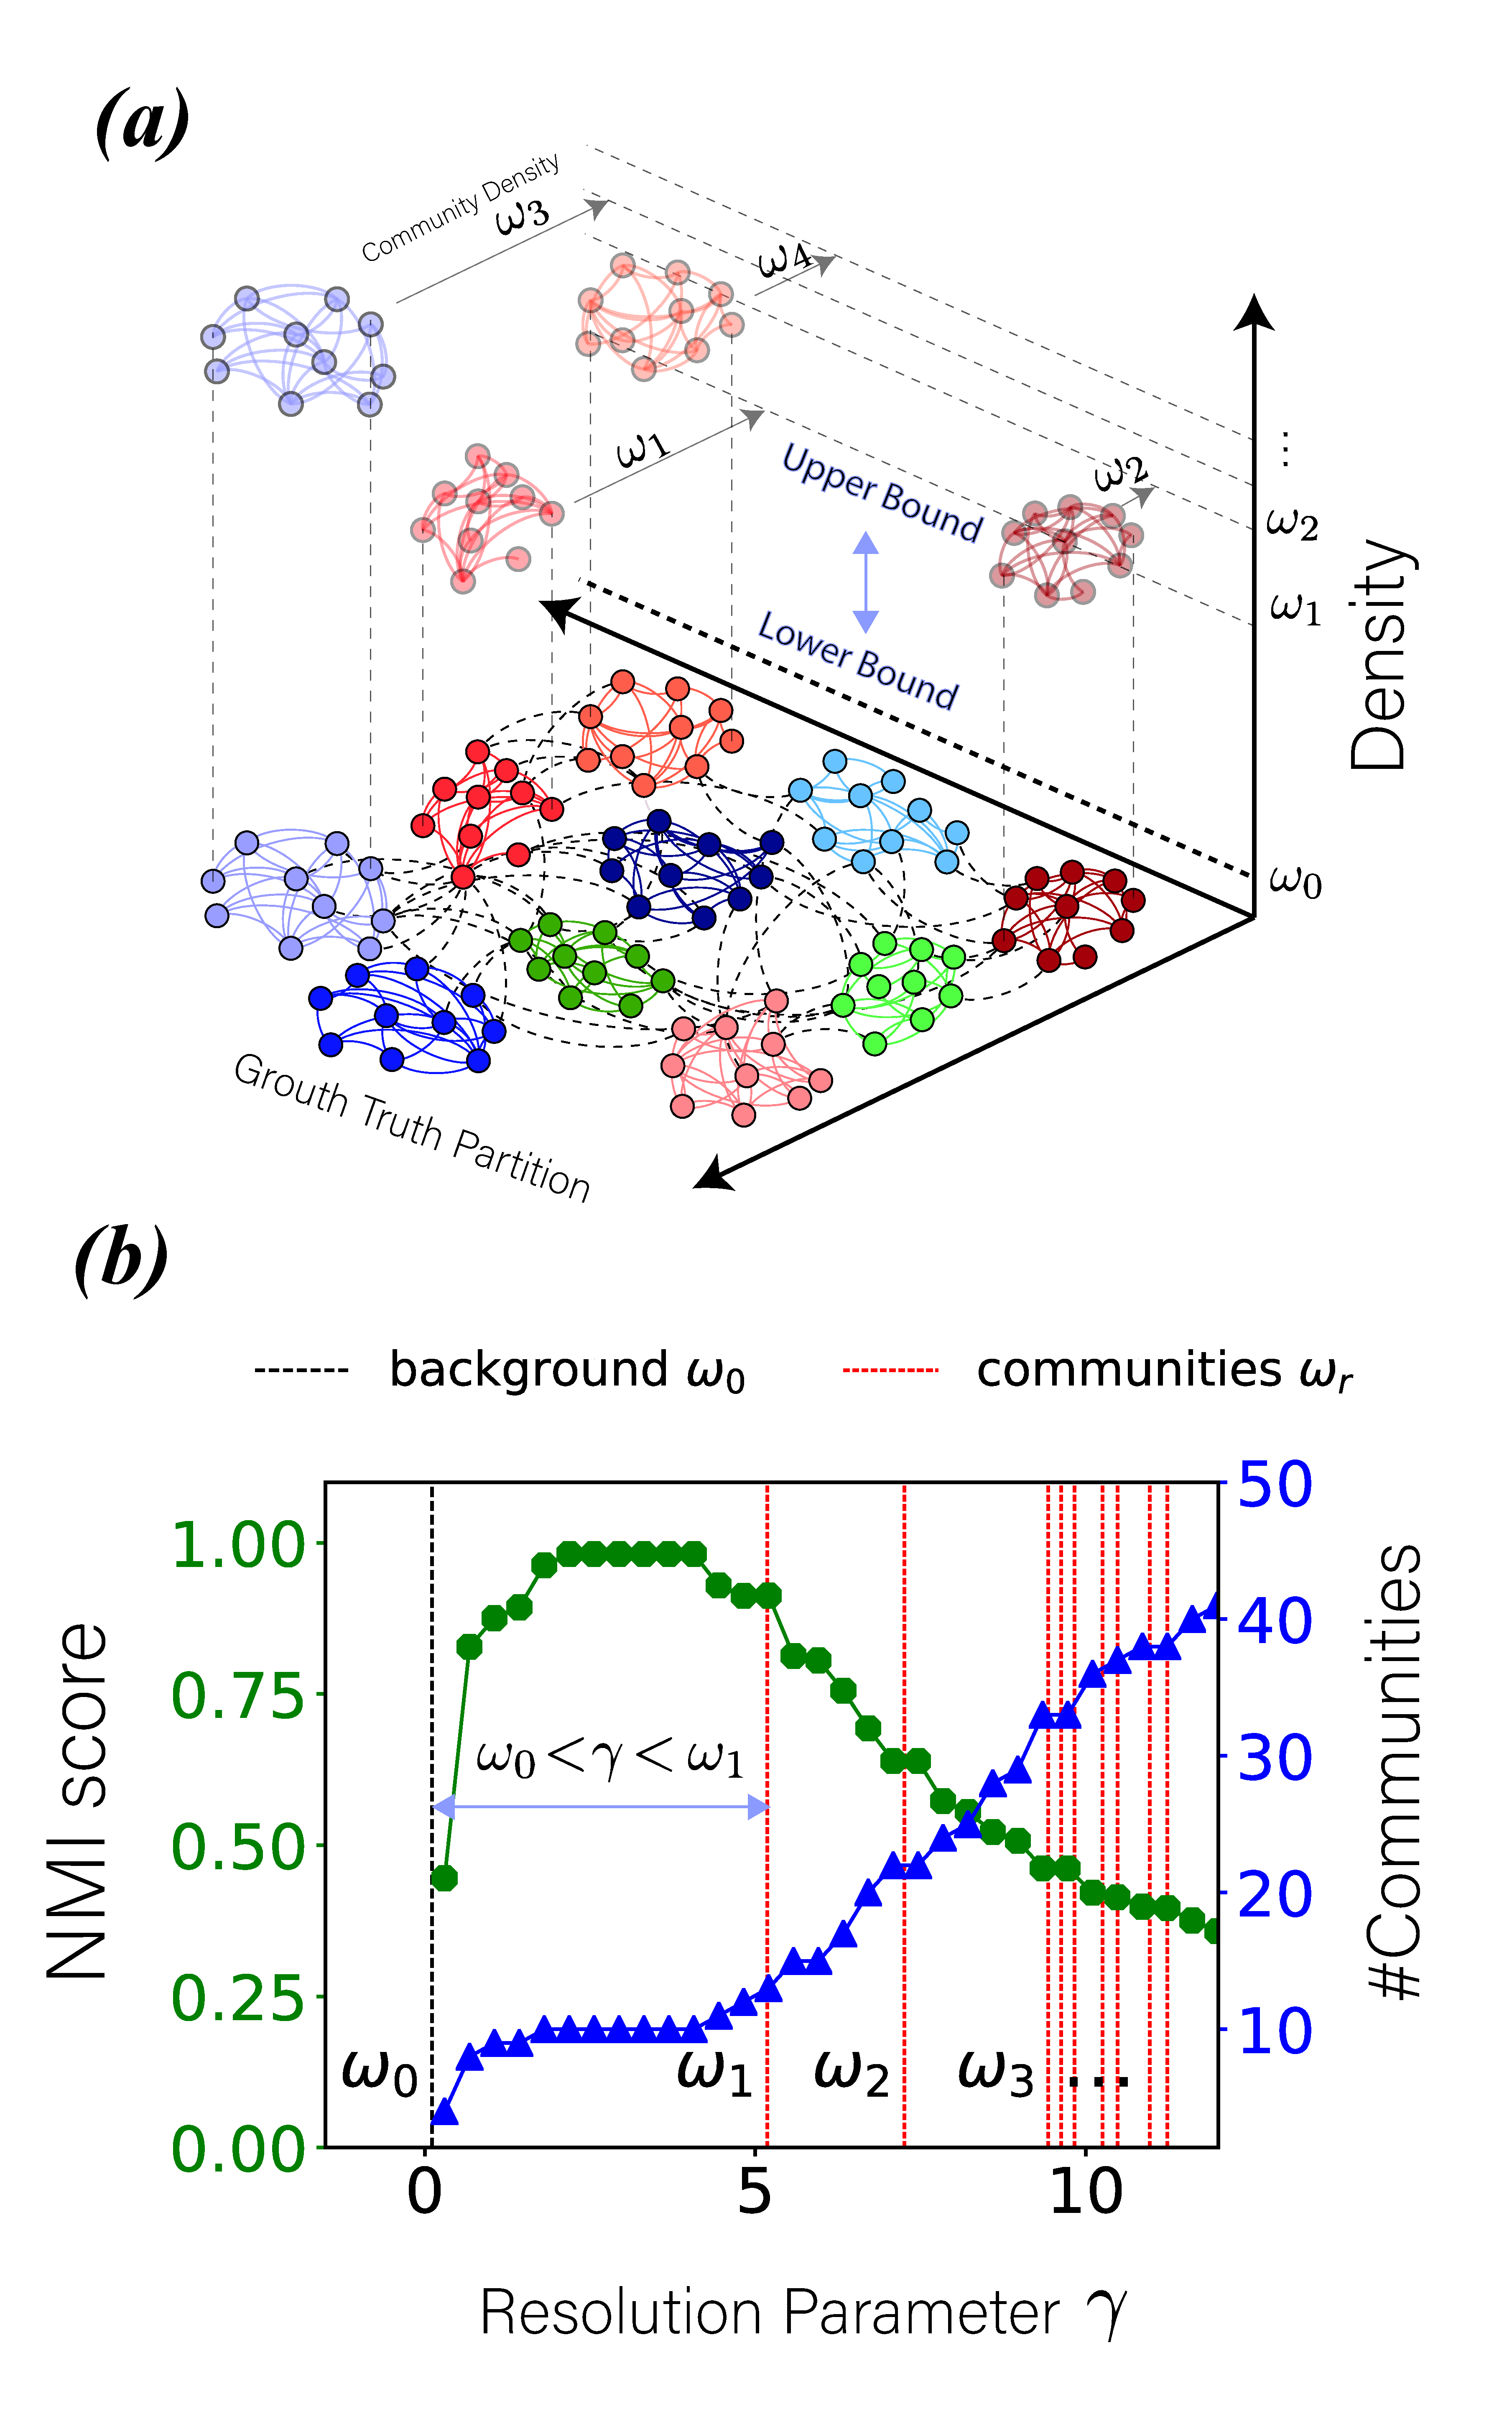
\includegraphics[width=0.6\textwidth]{img/chap2/Fig2.pdf}
    \caption{The generalized modularity performs well with resolution parameter in the interval $\gamma\in[1.8,4.2]$, matching the derived theoretical bound $\omega_0<\gamma<\omega_1$. When $\gamma$ approaches either side of the bound, the resolution scale is either higher or lower than desired. (a) Network structure and community {\it density} represented by the heights, the node color represents ground truth communities and inter-communities edges are in black dashed lines; (b) the NMI scores and the number of detected communities in relation to the resolution parameter.}
    \label{fig:gamma_error_exp}
\end{figure}

The asymptotic bounds also agree with the empirical observation made without any theoretical justification by the authors of~\cite{fenn2009dynamic,traag2013significant,mucha2010community}, that the most suitable values of the resolution parameter $\gamma$ occurs in the most stable plateaus in experiments. In addition, our results explain why \cite{newman2016equivalence} found that the statistical inference of the resolution parameter converges quickly to the desired value in small networks. It is because, once the resolution parameter falls into the range of $\omega_0<\gamma<\omega_1$, if feasible, the community detection results become stable and the inference algorithm immediately yields the final resolution parameter after this stage.

For a range of empirical networks of $n$ nodes and $m$ edges, including the Karate club network~\cite{zachary1977information}, the dolphin social network~\cite{lusseau2003bottlenose}, the network of interactions between fictional characters in the novel Les Miserables~\cite{newman2004finding} and the network of games between American college football teams in the year 2000~\cite{newman2004finding}, we compute the maximum-likelihood estimates of the background edge density $w_0$ and the lowest intra-community edge density $w_1$, fitting an extended planted partition model given the number of communities $q$ and the optimal value of $\gamma$ obtained by the statistical inference of~\cite{newman2016equivalence}. We compute the modularity maximization results with a total of $100$ different resolution parameters in the range $[0.2,3w_1/2]$ and compare these results with the communities produced with $\gamma$ from this range. The subrange which produces an NMI score higher than $90\%$ is shown in Table~\ref{tab:small_networks}. As shown in Fig.~\ref{fig:small_networks}, although these empirical networks are not generated by the extended planted partition model, the stable intervals of resolution parameter lie inside the asymptotic lower and upper bounds.

\begin{table}[]
    \centering
    \caption{The maximum-likelihood estimates of $w_0$ and $w_1$ and the interval of the resolution parameter that detects communities with NMI score larger than 90\% in a range of empirical networks of $n$ nodes and $m$ edges. The number of communities $q$ used for each network is the ground truth value generally accepted in the previous literature. The optimal $\gamma$ were published in~\cite{newman2016equivalence}.}
    \label{tab:small_networks}
    \begin{tabular}{ccccccc}
    \hline
    Network & n & m & q & $\gamma$ & $(\hat{w}_0,\hat{w}_1)$ & $90\%$ interval\\
    \hline
    Karate club & 34 & 78 &  2 & 0.78 & (0.26, 1.74) & (0.63, 1.37)\\
    Dolphin social & 62 & 159 & 2 & 0.59 & (0.12, 1.42) & (0.58, 2.0)\\
    Les Miserables & 77 & 254 & 6 & 1.36 &  (0.35, 2.83) & (1.15,  1.54)\\
    College football & 115 & 614 & 11 & 2.27 & (0.36, 5.11) & (1.78,5.61)\\
    \hline
    \end{tabular}
\end{table}


\begin{figure}[t!]
    \centering
    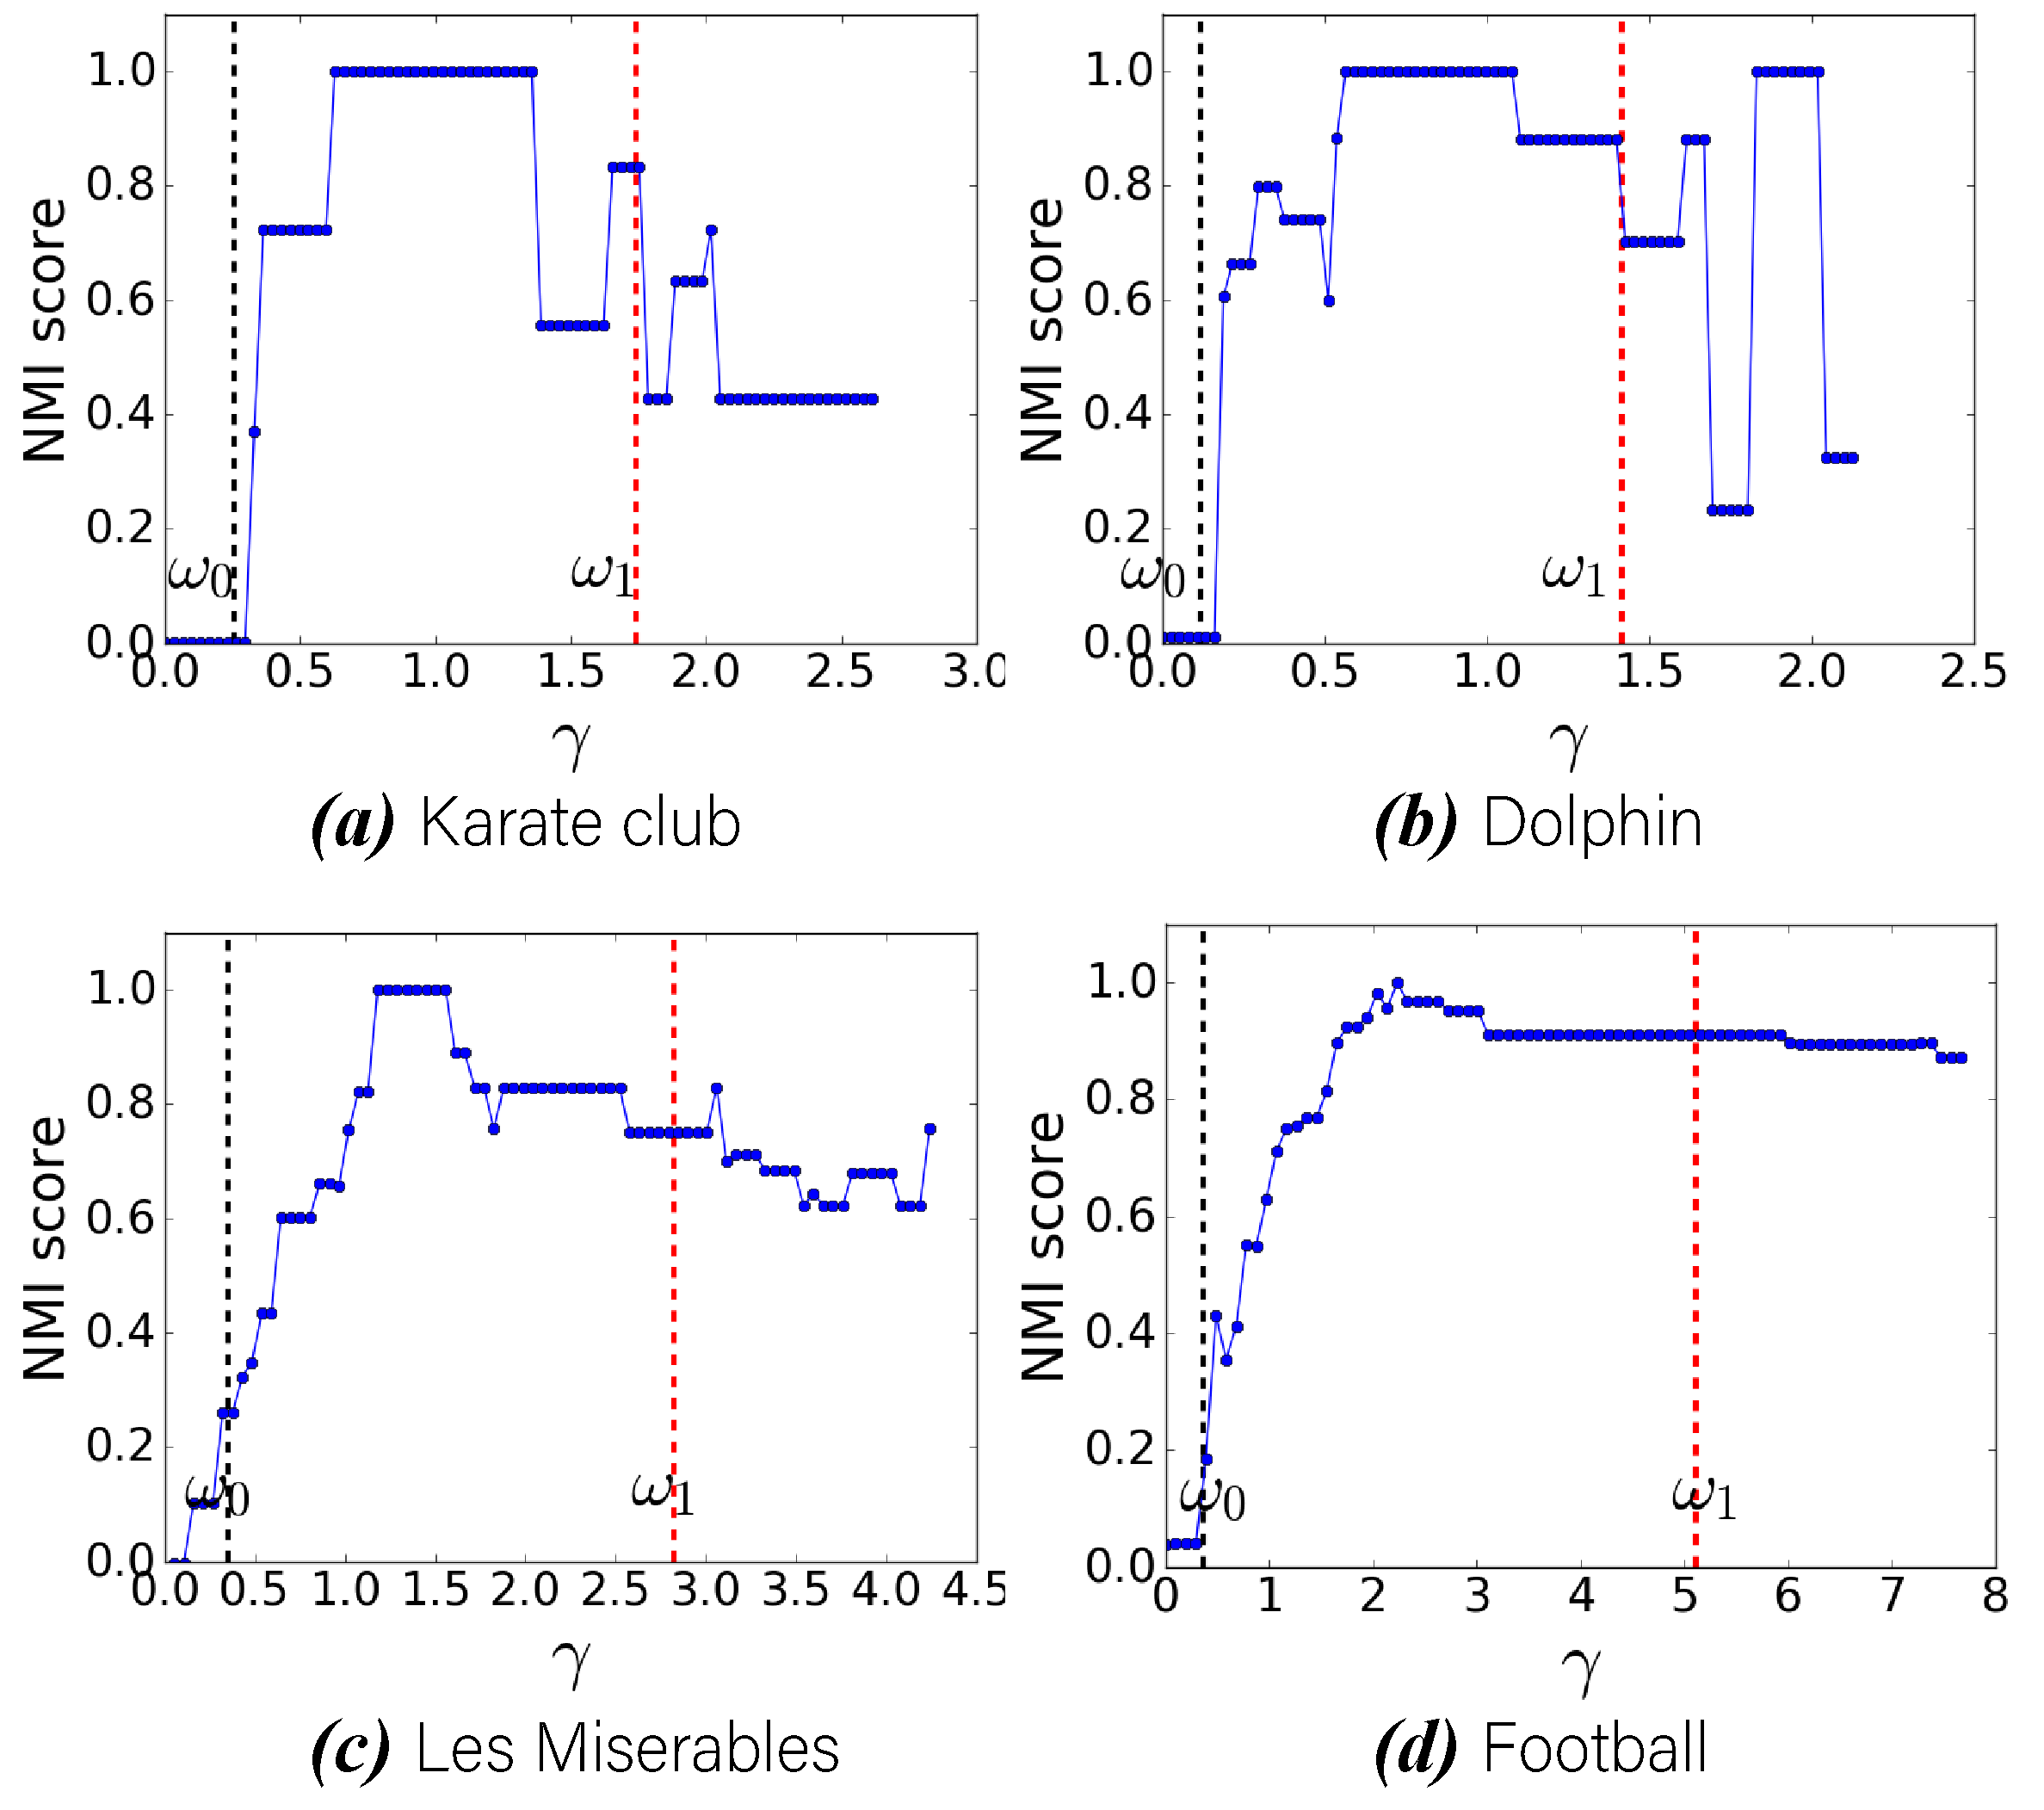
\includegraphics[width=0.8\textwidth]{img/chap2/Fig6.pdf}
    \caption{The alignment between the communities detected by generalized modularity maximization and the optimal $\gamma$ values listed in~\cite{newman2016equivalence}. Although the empirical networks are not generated by the extend planted partition model, maximizing the generalized modularity is optimal when the resolution parameter takes values that lie in the interval $[\omega_0, \omega_1]$. This phenomenon is also captured purely experimentally and without any theoretical justification in~\cite{fenn2009dynamic,mucha2010community,traag2013significant}.}
    \label{fig:small_networks}
\end{figure}


\section{Statistically significant community detection} \label{sec:2.4}
The planted partition model and its extension introduced here are all special cases of the stochastic block model. The derived asymptotic resolution bounds can be extended to the networks generated by the degree-corrected stochastic block model. Following the notations in~\cite{newman2016equivalence}, the number of edges between nodes $i$ and $j$ in the degree-corrected stochastic block model follows the Poisson distribution with the mean defined as 
\begin{equation} \label{eq:sbm_newman_definition}
\eta_{ij} = \omega_{g_i g_j} \frac{k_i k_j}{2m},
\end{equation}
where for node $l$, $g_l$ is the block assignment of this node, $k_l$ is its degree and $m$ is the total number of edges in the network.

The number of edges between two communities $r$ and $s$ in this case is approximated by 
\begin{equation} \label{eq:approx_out2}
    m_{rs} \approx \sum_{i\in r, j\in s} \omega_{rs} \frac{k_i k_j}{2m} = \omega_{rs} \frac{\kappa_r \kappa_s}{2m},
\end{equation}
where $\omega_{rs}$ denotes the (r, s)-th element of the {\it density} matrix. The number of edges between two subsets of nodes $t'$ and $t''=t - t'$ inside a community $t$ is approximated by
\begin{equation} \label{eq:approx_in2}
    m_{t't''} \approx \sum_{i\in t',j\in t''} \omega_{tt} \frac{k_i k_j}{2m} = \omega_{tt} \frac{\kappa_{t'} \kappa_{t''}}{2m},
\end{equation}
where $\omega_{tt}$ is the t-th diagonal element in the {\it density} matrix.

Using the same resolution inequality of Eq.~\ref{eq:resolution}, these approximations lead to the range
\begin{equation} \label{eq:sbm_bounds}
    \max_{r\neq s} \omega_{rs} < \gamma < \min_{r} \omega_{rr}
\end{equation}
within which a uniform $\gamma$ value avoids the resolution limit trap. 

In a network generated by the degree-corrected stochastic block model with $\omega_{rs} > \omega_{tt}$ for some $r \neq s$ and $t$, Eq.~\ref{eq:sbm_bounds} indicates that a uniform resolution parameter is not sufficient for the recovery of communities $r$, $s$ and $t$.

\begin{figure}
    \centering
    \includegraphics[width=.6\textwidth]{img/chap2/altitude.pdf}
    \caption{The plateaus problem is analogous to finding mountains that are located at different plateaus; using a single altitude either would miss the lower mountains, or would treat the higher peeks as one mountain. Specifically, when using resolution parameter $\gamma_l$, the left two high peeks P1 and P2 are considered one ``mountain" - two well-formed dense communities get merged because their inter-community edge density (illustrated by valley V1) is higher than $\gamma_l$. If we adopt a higher resolution parameter $\gamma_h$, the low peek P4 on the right gets ignored - a loose community gets split into multiple smaller clusters. Notably, this issue cannot be avoided as long as the valley V1 of the left two peeks P1, P2 is higher than the height of the right-most peek P4.}
    \label{fig:plateaus}
\end{figure}

The classical example of resolution limit trap is presented in~\cite{lancichinetti2011limits} where an undirected unweighted network contains three communities: two cliques and one ER random graph, and every two communities are connected by one single edge. Suppose each clique includes 6 nodes and the ER random graph contains 100 nodes and 956 edges. Given the three communities, the posterior estimation of the {\it density} matrix $\Omega$ of a stochastic block model, i.e., $\hat{\omega}_{rs} = \frac{2 m_{rs} m}{\kappa_r \kappa_s}$ for each communities $r$ and $s$, is
\begin{equation}
    \Omega = \begin{bmatrix}
    1.03	& 0.03  &	0.03	\\
    0.03	& 57.94 &	1.93  \\
    0.03	& 1.93  &	57.94 \\
    \end{bmatrix},
\end{equation}
where the first row and column corresponds to the random graph while the remaining rows and columns correspond to the two cliques respectively. There is no suitable resolution parameter $\gamma$ to detect three communities in this case because the {\it density} parameter for the edges between two cliques $1.93$ is larger than the {\it density} parameter for the edges inside random graph $1.03$. When applying generalized modularity maximization, adopting a resolution parameter larger than $1.93$, makes it likely that two cliques will be detected, but the random graph will get split into smaller communities. On the other hand, a resolution parameter within $[1.03, 1.93]$ preserves the random graph as one complete community, but the two clique gets merged into one community.

\begin{figure}
    \centering
    \includegraphics[width=8cm]{img/chap2/gamma_error.pdf}
    \caption{Resolution limits of the generalized modularity can be explained by the relations between the values of the density parameters of stochastic block models. Given two disjoint subgraphs A and B such that the inter-community edge density $\omega_{a0}$ in subgraph A is larger than the intra-community edge density of some community in subgraph B, no suitable resolution parameter $\gamma$ exists because Split Error and Merge Error cannot be resolved at the same time. Split Error occurs when the resolution parameter $\gamma_h$ is larger than the inter-community edge density of a subgraph A, because the community $b_1$ with the intra-community density smaller than $\gamma_h$ will be spread among multiple clusters; Merge Error occurs when the resolution parameter $\gamma_l$ is smaller than $\omega_{a0}$ so the communities in subgraph A will be merged into one community.}
    \label{fig:gamma_error}
\end{figure}

The issue is analogous to finding mountains that are located at different plateaus as shown in Fig.~\ref{fig:plateaus}; using a single altitude either would miss the lower mountains, or would treat the higher peeks as one mountain. Specifically, when using resolution parameter $\gamma_l$, the left two high peeks in Fig.~\ref{fig:plateaus} are considered one ``mountain" - two well-formed dense communities get merged. If we adopt a resolution parameter $\gamma_h$, the low peek on the right gets ignored - a loose community gets split into multiple smaller clusters. Notably, this issue cannot be avoided as long as the valley of the left two peeks is higher than the height of the right-most peek. 

More formally, given the {\it density} matrix of a degree-corrected stochastic block model and a set of communities $S=\{r\}$, the sub-matrix $\Omega_{S,S}$ formed by the rows and columns in $r\in S$ corresponds to a subgraph in the networks. Suppose subgraphs A and B have the inter-communities {\it density} parameter $\omega_{w_{a0}}$ and $\omega_{w_{b0}}$ respectively. In Fig.~\ref{fig:gamma_error}, using $\gamma_h$ causes {\it Split Error} which splits some community with $\omega_{b1} < \gamma_h$ in  B while using $\gamma_l$ causes {\it Merge Error} which merges all communities in subgraph A.

This problem is more common in large networks than in small ones, as large networks are more likely to have inhomogeneous subgraphs in different regions. For this reason, a uniform resolution limit parameter is not sufficient to resolve communities located at different ``plateaus''. Motivated by this ``plateaus'' phenomenon, we propose a multi-scale community detection algorithm which gradually increases the resolution parameter to detect community in local subgraphs.

We propose an agglomerative heuristic algorithm which recursively divides the network into subgraphs to detect communities at different scales. At each level of recursion, the algorithm applies a resolution parameter $\gamma < 1$ in attempt to avoid inappropriately splitting of loose communities. But it is likely to merge inappropriately small well-formed communities into large ones. Therefore, the discovered subgraphs are then passed to the next level of recursion to further detect communities with higher edge {\it density} parameter. This idea is illustrated in Fig.~\ref{fig:plateaus} where the peeks located at a higher plateaus need a high altitude $\gamma_h$ for each to have its own community.

The remaining challenge is to determine when to terminate the recursion. As the network breaks into smaller subgraphs recursively, the algorithm should stop when there is actually only one community in each subgraph. Indeed, one can always increase the resolution parameter to detect higher resolution communities in this subgraph. But it does not mean the current subgraph always contains community structures. For instance, a Erdos-Renyi random graph~\cite{erdHos1960evolution} can be partitioned into communities as long as the resolution parameter is high enough. However, we do not claim that Erdos-Renyi graph has community structures.

To ensure the detected communities are meaningful, we apply a {\bf hypothesis testing framework} to ensure the significance of the partition. The \textit{null} model $H_0$ here is defined as a simplified version of the degree-corrected planted partition model in which only one community exists, and the more general, nesting alternative $H_1$ is defined as the degree-corrected planted partition model whose log-likelihood is represented by Eq.~\ref{eq:modularity} given the current partition $\bf g$. 

The {\it null} model $H_0$ here is a special case of the degree-corrected planted partition model~\cite{newman2016equivalence}. The number of edges between nodes $i$ and $j$ follows the Poisson distribution with mean
\begin{equation}
    \eta_{ij} = \omega \frac{k_i k_j}{2m},
\end{equation}
where $\omega$ is a model parameter independent of the block assignments. Hence, we can consider this model as the degree-corrected planted partition model with only one community and the $\omega$ is the corresponding {\it density} parameter. The log-likelihood of this \textit{null} model can be simplified from Eq.~\ref{eq:ll} to the following
\begin{equation} 
\begin{split}
    \log P_{\text{null}}({\bf A}|\omega) &= \frac{1}{2} \sum_{ij} \left[ A_{ij} \log \left(\omega\frac{k_i k_j}{2m} \right) - \omega\frac{k_i k_j}{2m} \right] \\
                           &= m \left(\log w - w\right) + \sum_i k_i \log k_i - m \log \left(2m\right) .
\end{split}
\end{equation}
Taking the first-order derivative of the log-likelihood above over $\omega$, it is easy to obtain the maximum likelihood estimate $\hat{\omega} = 1$, hence the posterior log-likelihood can be written as
\begin{equation} \label{eq:null_ll}
\log P_{\text{null}}({\bf A}) = - m + D,
\end{equation}
where $D$ is the constant term given in Eq.~\ref{eq:BCD}, which actually can be cancelled eventually in the test statistic as shown below.

It is worth noting that the {\it null} model defined here is similar to the configuration model~\cite{molloy1995critical}, but they are not exactly equivalent. The configuration model~\cite{molloy1995critical} is a random graph model which assumes the edges are placed randomly between the nodes, while the degree of every node after such randomization is equal to the corresponding value in the original network. The network generation process in the configuration model can be understood as follows: The degrees of the vertices are represented as the number of half-links or stubs. These stubs are randomly paired with each other to create the edges. Hence, the configuration model produces an ensemble of graphs with the exact degree sequence as in the original network. The number of edges between nodes $i$ and $j$ averaged over the ensemble of graphs generated in this way is equal to $\frac{k_i k_j}{2m}$ where $m$ is again the total number of edges in the original network and $k_l$ is the degree of node $l$. In the {\it null} model defined here, when the $\omega$ parameter takes the MLE value $\hat{\omega} = 1$, the expected number of edges between nodes $i$ and $j$ is also $\frac{k_i k_j}{2m}$. But this {\it null} model allows multi-edges and self-edges (edges connecting a node to itself). The expected degree of the node $i$ in the {\it null} model is $\sum_j \frac{k_i k_j}{2m} = k_i \frac{\sum_j k_j}{2m} = k_i$.

In general, the alternative model $H_1$ splitting a network into multiple communities should fit better to the observed network than the {\it null} model does because the alternative model involves many more model parameters. The log-likelihood of the degree-corrected planted partition model, $\log P_{\text{pp}}$, is supposed to be higher than the log-likelihood of the {\it null} model, $\log P_{\text{null}}$ as defined in Eq.~\ref{eq:modularity}. Therefore, we use the log-likelihood ratio statistic (LLR)~\cite{ghosh1984asymptotic} as a test statistic to measure their difference. Given a partition of the network $\bf g$, the LLR is written as
\begin{equation} \label{eq:-2ll}
    \begin{split}
    \Lambda_{\bf g} &= -2 \log \frac{P_{\text{null}}({\bf A})}{P_{\text{pp}}({\bf A};\hat{\Omega}_{\bf g},{\bf g})} \\
                      &= 2 \left[ \log P_{\text{pp}} \left( {\bf A};\hat{\Omega}_{\bf g},{\bf g} \right) - \log P_{\text{null}} \left( {\bf A} \right) \right],
    \end{split}
\end{equation}
where $\hat{\Omega}$ is the posterior most-likely {\it density} parameters estimated from the given partition $\bf g$. The log-likelihood ratio statistic is equal to twice the difference between the log-likelihood of two models, $\log P_{\text{pp}}$ and $\log P_{\text{null}}$. 

It is worth noting that the partition $\bf g$ is detected by the generalized modularity maximization and used to compute $\log P_{\text{pp}}({\bf A};\hat{\Omega}_{\bf g},{\bf g})$ in our case. A low resolution parameter $\gamma$ value is used for the generalized modularity maximization here because it is likely to result in a small number of communities, limiting the number of parameters in the alternative model $H_1$. Hence, it prevents the $H_1$ model from overfitting. Most importantly, this choice avoids the multiple re-estimation of $\gamma$, which is computationally expensive because it needs to maximize the generalized modularity over the same network many times with different $\gamma$ values~\cite{newman2016equivalence}. In practice, we choose a $\gamma$ value slightly smaller than $1$ in the experiments.

Plugging the specific expression of the log-likelihoods of these two competing models, Eq.~\ref{eq:modularity} and Eq.~\ref{eq:null_ll}, into Eq.~\ref{eq:-2ll} yields the test statistic in a simple form
\begin{equation} 
    \begin{split}
    \Lambda_{\bf g} &= 2 \left[ B \cdot Q \left(\hat{\gamma}, {\bf g} \right) + C + m \right] \\
        &= m \left[\log \frac{\hat{\omega}_1}{\hat{\omega}_0} \cdot Q \left(\hat{\gamma}, {\bf g} \right) + \left(\log \hat{\omega}_0 - \hat{\omega}_0 \right) + 1 \right],
    \end{split}
\end{equation}
where the constants $B$ and $C$ are defined in Eq.~\ref{eq:BCD} but the parameters $\omega_1$ and $\omega_0$ take their MLE values, and $Q(\hat{\gamma}, {\bf g})$ is the generalized modularity of the partition $\bf g$ with a resolution parameter $\hat{\gamma}$ defined by posterior maximum likelihood estimate, $\hat{\omega}_0$ and $\hat{\omega}_1$ are the {\it density} parameters obtained by the posterior maximum likelihood estimation given partition $\bf g$. With $\hat{\gamma}$ and ${\bf g}$, it takes $O(m)$ time to compute $Q(\hat{\gamma}, {\bf g})$ where $m$ is the total number of edges in the network. Given the modularity $Q(\hat{\gamma}, {\bf g})$, the LLR test statistic can be computed in constant time.

In general, the alternative model $H_1$ splitting a network into multiple communities should perform at least as well as the \textit{null} model, because the alternative model involves many more model parameters, i.e. the {\it density} matrix $\Omega$. $H_1$ is accepted when the fit is significantly better, i.e. $\Lambda_{\bf g}$ is large enough. Such significance is measured by the \textit{p-value} of $\Lambda_{\bf g}$ defined as
\begin{equation}
    \textit{p-value} = P [\Lambda_{\text{null}} > \Lambda_{\bf g}],
\end{equation}
where $\Lambda_{\text{null}}$ is the corresponding log-likelihood value under the {\it null} hypothesis, which can be computed numerically by sampling a series of \textit{null} networks generated by the {\it null} model. If the {\it p-value} is smaller than the significance level, the {\it null} hypothesis is rejected and the algorithm does hypothesis testing on the resulting communities; Otherwise, the algorithm returns the current subgraph as one single community and stops the current recursion branch. The hypothesis testing procedure is summarized below:
\begin{itemize}
    \item Maximize the generalized modularity with a predefined $\gamma < 1$ to obtain partition $\bf g$.
    \item Estimate the {\it density} parameters $\hat{\Omega} = \{\hat{\omega}_0, \hat{\omega}_1\}$ of degree-corrected planted partition model by Eq.~\ref{eq:update_omega} and the corresponding resolution parameter $\bf \hat{\gamma}$ by Eq.~\ref{eq:gamma_mle}. Then compute the generalized modularity $Q(\hat{\gamma}, {\bf g})$ so the log-likelihood ratio test $\Lambda_{\bf g}$ can be obtained.
    \item Generate a series of \textit{null} networks via the {\it null} model. Compute $\Lambda_{\text{null}}$ for each \textit{null} network, output the fraction of $\Lambda_{\text{null}}$s which are larger than $\Lambda_{\bf g}$ as the \textit{p-value}.
    \item If the {\it p-value} is smaller than the significance level, reject $H_0$ and continue partitioning the subgraph. Otherwise, accept $H_0$ and return the current subgraph as a community.
\end{itemize}

It is worth noting that, according to the Wilks' theorem~\cite{wilks1938large}, when the sample size, i.e. the number of sampled {\it null} networks, approaches infinity, the log-likelihood ratio test statistic as defined in the form of Eq.~\ref{eq:-2ll} is asymptotically chi-squared distributed when the $H_0$ hold true. We can actually avoid enumerating a large set of {\it null} networks to calculate the {\it p-value}. Instead, given $\Lambda_{\bf g}$, the {\it p-value} can be directly approximated using the chi-squared distribution. However, in practice, the quality of $\bf g$ also influence the test statistic $\Lambda_{g}$. We observed that modularity maximization over a larger network often detects better $\bf g$ than over smaller ones, resulting in large test statistic $\Lambda_{g}$. Therefore, we find it more computationally efficient to terminate the current recursion branch when $\Lambda_{\bf g} < \tau * n_{sub}$ where $\tau$ is a constant value and $n_{sub}$ is the number of nodes in the currently considered subgraph. The accurate calculation of {\it p-value} by sampling {\it null} networks can still be used for relatively small network when needed.

To evaluate the performance of the proposed multi-scale community detection algorithm, we compare it with the state-of-art greedy modularity maximization algorithm, Fast Greedy~\cite{clauset2004finding}, on several real and synthetic networks. For the networks with pre-defined ground truth communities, the quality of the detected communities are evaluated by the Normalized Mutual Information (NMI) and Adjusted Rand Index (ARI) metrics which requires ground truth communities. Besides, we also measure the distribution of the community sizes which usually reflects the resolution limits problem because modularity maximization either combines smaller well-formed communities into bigger ones or splits larger well-formed communities into smaller ones. The definition of the two quality metrics mentioned above are given below.

One of the standard sources of community structures for the evaluation of community detection algorithms is the LFR benchmark~\cite{lancichinetti2008benchmark} which generates networks based on a set of pre-defined ground truth communities. In so generated networks, both the degree and community size distributions follow the power law. The main benefit of using LFR benchmark is that the ground truth communities are known. The generated networks vary with the following three parameters: $\gamma$ which is an exponent of the node degree in the power law distribution, $\beta$ which is an exponent of the community size in the power law distribution, and $\mu$ which is the {\it density} parameter that defines the fraction of all edges which have both endpoints inside the same community. 

In our experiments, the networks generated by the LFR benchmarks have the average node degree of 9.3 and the numbers of nodes ranging from 6,000 to 11,000. The exponents $\gamma$ and $\beta$ are set to 3.0 and 2.0 respectively and the {\it density} parameter $\mu$ is equal to 0.25. We evaluate the modularity maximization performance using the Fast Greedy algorithm~\cite{clauset2004finding}. The results are measured by the NMI and ARI metrics as shown in Table~\ref{tab:1}. The number of communities as a function of their sizes is plotted in Fig.~\ref{fig:5}. One notable difference between the community detection results is that the modularity maximization merges smaller communities into larger ones so there is fewer small communities in the results than in the ground truth. This is the main reason why modularity maximization does not perform as well as the proposed multi-scale community detection which recursively divides a large community into small ones until the probability that it contains communities becomes statistically insignificant.

\begin{table}[]
\centering
\caption{Performance of multi-scale community detection compared to the Fast Greedy~\cite{clauset2004finding} modularity maximization algorithm on the LFR benchmark networks. Note large increase in value of metrics for multi-scale algorithm, at least 38\% for NMI and 240\% for ARI}
\label{tab:1}
\begin{tabular}{ccccc}
\hline
\multirow{2}{*}{\#Nodes} & \multirow{2}{*}{\#Edges} & \multirow{2}{*}{Metric} & \multirow{2}{*}{Fast Greedy} & \multirow{2}{*}{Multi-scale} \\
                  &                   &                  &            &                           \\
\hline

\multirow{2}{*}{5000} & \multirow{2}{*}{23436} & ARI     &  0.20368   &  0.69378                \\
                  &                   &          NMI     &  0.60266   &  0.83706                         \\
\multirow{2}{*}{7000} & \multirow{2}{*}{31546} & ARI     &  0.12377   &  0.71148                \\
                  &                   &          NMI     &  0.62044   &  0.87240                         \\
\multirow{2}{*}{9000} & \multirow{2}{*}{41595} & ARI     &  0.11038   &  0.74156               \\
&                   &          NMI     &  0.59043   &  0.87355                        \\
\multirow{2}{*}{11000} & \multirow{2}{*}{51430} & ARI     &  0.12701   &  0.75043               \\
&                   &          NMI     &  0.56224   &  0.86722              \\          
\hline
\end{tabular}
\end{table}

\begin{figure}[!ht]
    \centering
    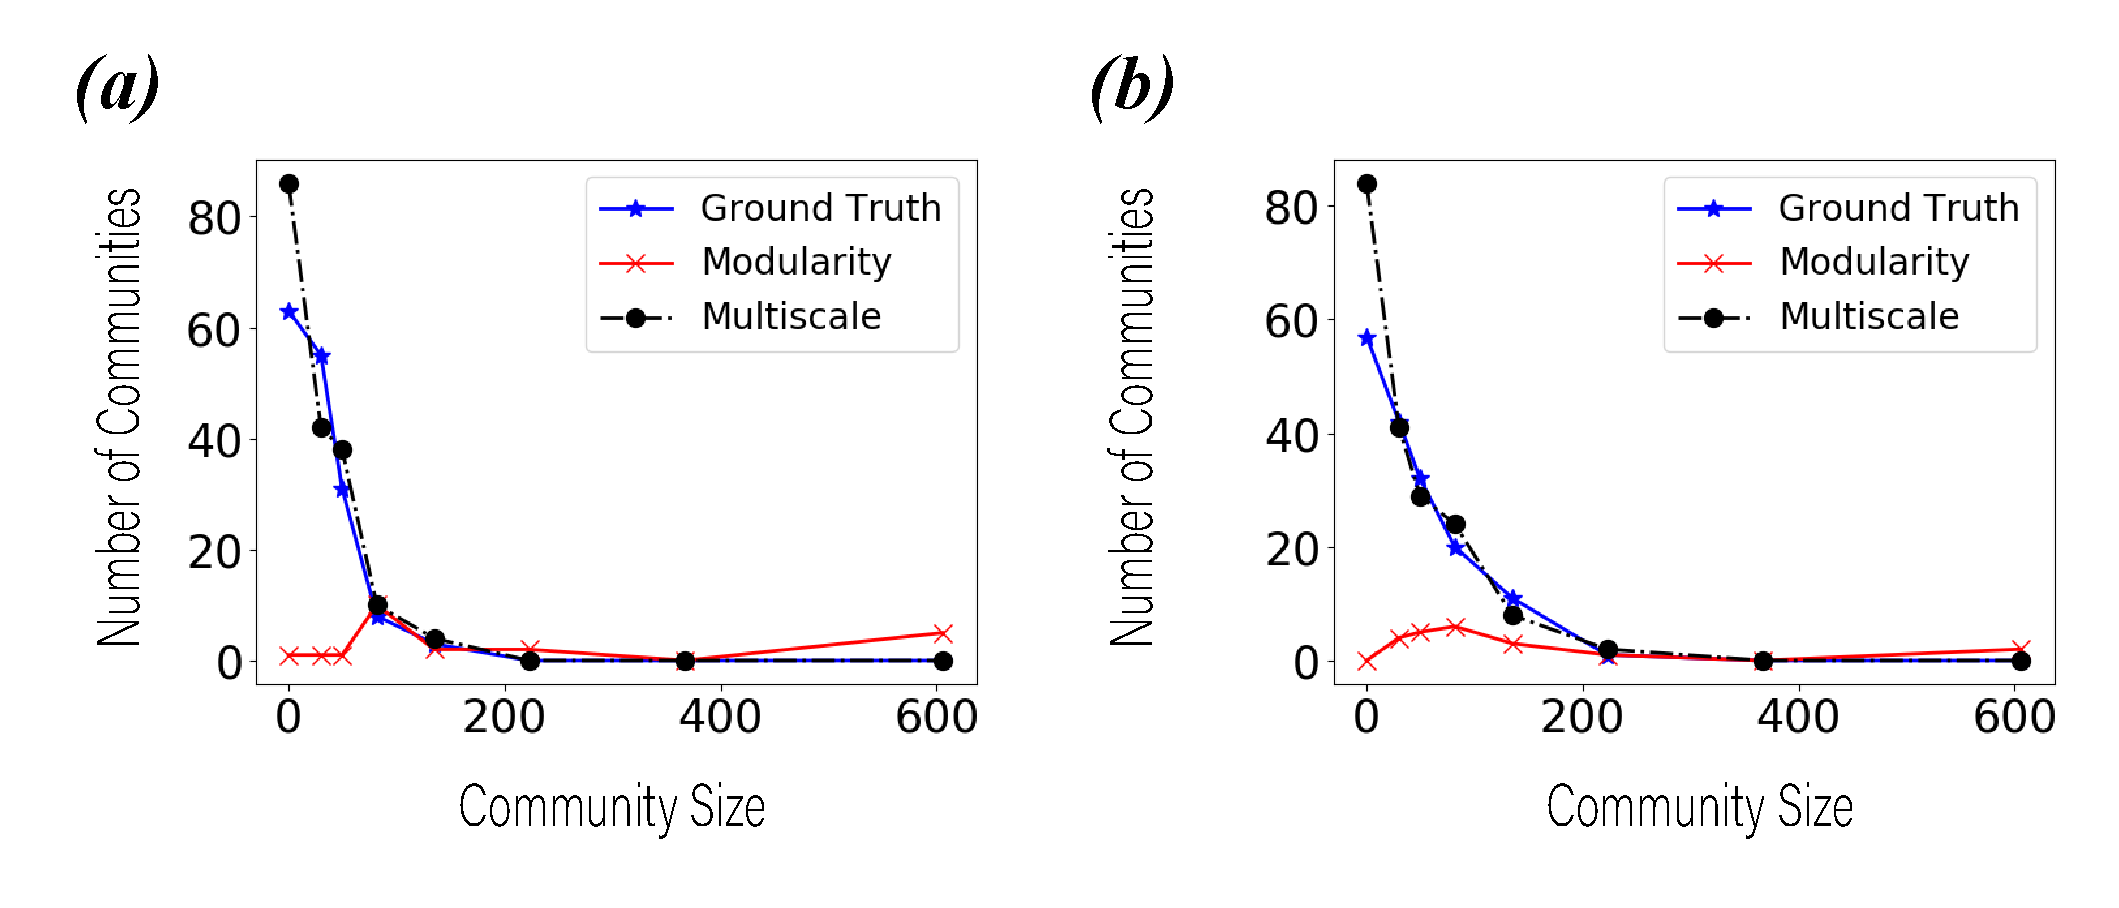
\includegraphics[width=0.9\textwidth]{img/chap2/Fig5.pdf}
    \caption{Histogram of detected community sizes using the state-of-the-art modularity maximization algorithm, Fast Greedy~\cite{clauset2004finding}, and the proposed multi-scale modularity maximization approach. This approach detects fewer small communities and more large communities compared to the ground truth due to the resolution limit problem. In contrast, the multi-scale approach detects the numbers of communities of over wider range of sizes. (a) LFR benchmark network with 7000 nodes (b) LFR benchmark network with 11,000 nodes.}
    \label{fig:5}
\end{figure}

The American college football network~\cite{evans2010clique} consists of 115 nodes representing college football teams playing in a league with 11 conferences. Every edge in the American college football network denotes the positive number of games played by two teams in the year 2000 season. According to~\cite{evans2010clique}, each of the 11 college football conferences active at the time gets identified as one community because teams within a conference play more frequently with each other than with teams from other conferences. There are 8 independent teams (not members of any conference), each forming a single community. 

\begin{figure}
    \centering
    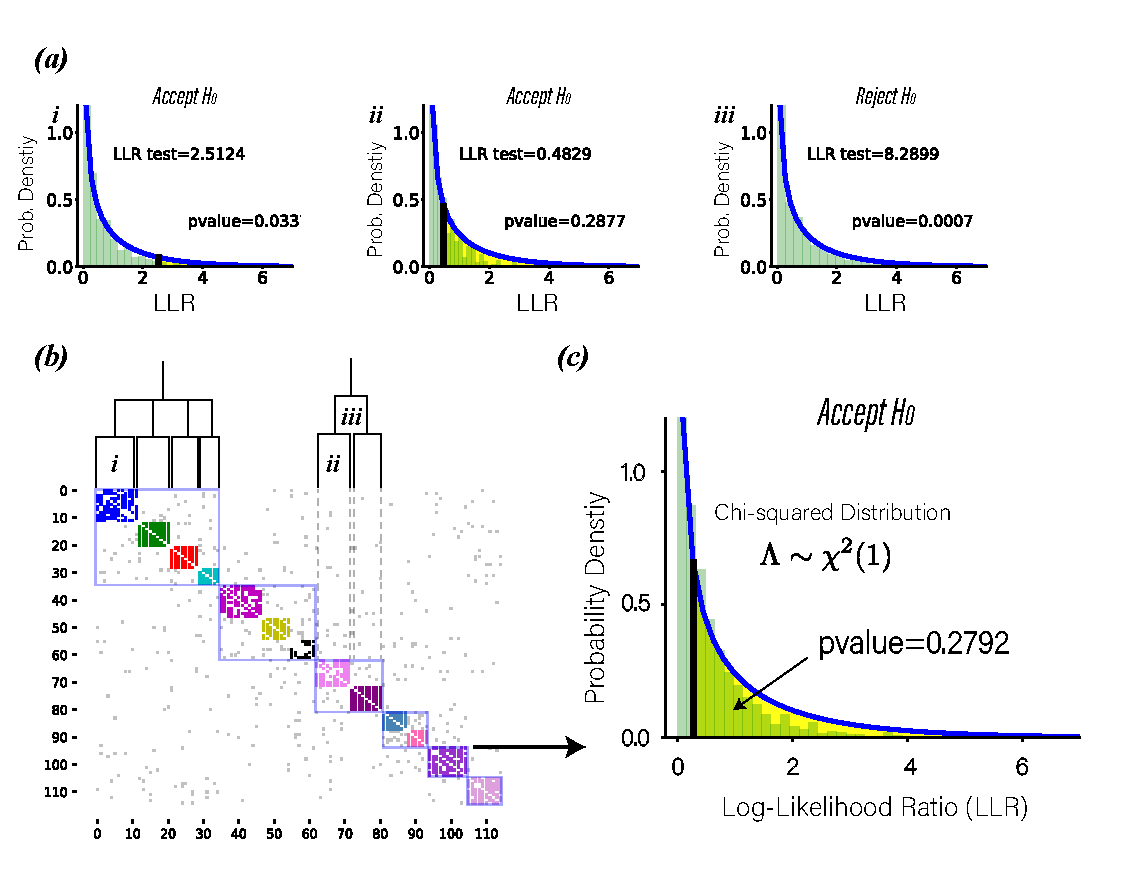
\includegraphics[width=0.8\textwidth]{img/chap2/football.pdf}
    \caption{Illustration of the multi-scale community detection in the American college football network~\cite{evans2010clique}. (a) Three different hypothesis testing cases are: in cases (i) and (ii) the {\it null} hypothesis is accepted because statistically significant community has been found while in case (iii) the {\it null} hypothesis is rejected because the subgraph actually consists of two smaller communities. (b) The edge matrix where each dot indicates the one edge. Different colors define final communities detected by multi-scale community detection, while the rectangles show the communities detected at the first level. (c) A well-formed community passes the statistical significance test at the first level, and thus avoids further splitting. The green histogram shows the distribution by sampling {\it null} networks, the blue curve indicate the chi-squared distribution, and the size of the yellow area corresponds to the {\it p-value}.}
    \label{fig:football_pvalues}
\end{figure}



Fig.~\ref{fig:football_pvalues} illustrates the steps of significance testing of the communities at two different levels. The generalized modularity with a predefined resolution parameter $\gamma=0.9$ is maximized to obtain partitions. As shown in Fig.~\ref{fig:football_pvalues}(b), at the first level, the networks is partitioned into 6 communities covered by the rectangles - some correspond to the well-formed ones because their community {\it densities} are larger than the resolution bound; the others, however, consist of multiple well-formed but smaller communities, each represented by an unique color. Then, the algorithm does hypothesis testing given the partition at the first level - it estimates the corresponding posterior maximum-likelihood estimates of {\it density} parameters $\hat{\Omega}$ and evaluate the log-likelihood ratio test $\Lambda_{\bf g}$. Then, the algorithm generates a series of \textit{null} networks via the configuration model, given the degree sequence of the network. Since the {\it p-value} is smaller than the significance level $0.01$ chosen here, which is typically used for such tests, we reject the {\it null} hypothesis $H_0$ and continue partitioning the each of the 6 communities. At the second level, each individual community is treated as a subgraph, and the same generalized modularity maximization procedure is repeated on each of them again.
The second community at the bottom right corner has a high community {\it density}, thus, the {\it null} hypothesis gets accepted with high p-value of $0.2792$, in case (i) and similarly in case (ii).
However, in case (iii), as shown in Fig.~\ref{fig:football_pvalues}(a)(iii), the {\it p-value} $0.0007$ is much smaller than the significance level of $0.01$ used here. Therefore, the multi-scale community detection algorithm rejects $H_0$ and further splits that ill-formed community into two smaller ones. The modularity maximization conducted by Fast Greedy obtains 6 communities similar to the ones covered by the six rectangles in Fig.~\ref{fig:football_pvalues}(c) and it obtains a NMI score of $0.5572$. The proposed multi-scale community detection algorithm finds $13$ communities, achieving the NMI scores of $0.8728$.


\section{Regularized Stochastic Block Model} \label{sec:2.5}
As defined in previous literatures~\cite{newman2004finding,fortunato2010community}, the assortative structures correspond to the traditional community structures, nodes are more frequently connected with each other inside communities than with the rest of the network. The disasortative structures do not satisfy this condition. For example, the core-periphery structures~\cite{borgatti2000models} divides the networks nodes into the core part, where nodes are often the hubs of the networks, and the periphery part, where nodes of low-degree connect to the core nodes. This is an advantage of the degree-corrected stochastic block model because it allows the discovery of the structures with different mixing patterns. However, when searching for the weak assortative community structures, the inference algorithm may still return the disassortative structure\cite{decelle2011asymptotic} instead.

We generate synthetic networks using the degree-corrected stochastic block model with a block assignment $\{g_i\}$ and the parameters $\omega_{rs}$ chosen for the assortative communities as follows
\begin{equation} \label{eq:synthetic}
\omega_{rs}=
    \begin{cases}
    &\gamma \omega_{0} \quad \quad  \text{ if  } r=s,\\
    &\omega_{0} \quad \quad \quad  \text{if  } r\neq s.
    \end{cases}
\end{equation}
where a large value of $\gamma$ results in strong community structure while $\omega_{0}$ controls the sparsity of the network. The degree sequence is drawn from a power-law distribution with exponent $2.5$, and the block assignments are randomly assigned, but each block is of the same size.

\begin{figure*}[!htb]
\centering
\begin{subfigure}{.5\textwidth} 
\centering
\includegraphics[width=.99\linewidth]{img/chap2/opt_figure_dcsbm.jpg}
\caption{Local optima of log-likelihood}
\end{subfigure}
\begin{subfigure}{.45\textwidth} 
\centering
\includegraphics[width=.99\linewidth]{img/chap2/dcsbm_converge2.png}
\caption{Convergence}
\end{subfigure}
\caption{The convergence of 20 Markov Chain Monte Carlo (MCMC) trials for the degree-corrected stochastic block model. The local optimum $A$ found by MCMC represents the assortative communities, whereas there are other local optima representing disassortative structures such as point B. \textbf{(a)} Multiple locally optimal partitions discovered by the MCMC inference for degree-corrected stochastic block model; \textbf{(b)} 2 out of the 20 MCMC trials find the most likely and sought-after assortative partition, while the other trials get trapped at the local optima. The matrix $M_{rs}$ indicates the number of edges between every pair of blocks.}
\label{fig:dcsbm_3dscatter}
\end{figure*}

Given the synthetic networks produced by the degree-corrected stochastic block model, we infer the block assignment $\{g_i\}$, recovering the parameters used for its generation. Specifically, the number of communities is set as two for both the generation and recovery. To generate samples, the degree-corrected stochastic block model uses $\omega_{0}=0.01$ and $\gamma=10$. Each of the two blocks contains $10$ nodes. We scatter the sampled partitions on the x-y plane in Figure~\ref{fig:dcsbm_3dscatter} and the z-axis indicates the log-likelihood of the corresponding partitions. We adapt the Markov chain Monte Carlo (MCMC) algorithm~\cite{nasrabadi2007pattern,peixoto2014efficient} to infer the block assignment of the stochastic block model and its extensions. The MCMC algorithm~\cite{peixoto2014efficient} samples the distribution of all possible block assignments in the network partitions space. For each trail, the algorithm starts from a random partition and iteratively, with certain probability, traverse to an adjacent partition. An entire MCMC sweep of all nodes in the network requires $O(E)$ operations where $E$ is the number of edges in the networks~\cite{peixoto2014efficient}. The mixing time of the MCMC algorithm depends on the specific input network and the starting point. The details of the MCMC algorithm are discussed in the Supplementary Information.

Figure~\ref{fig:dcsbm_3dscatter} shows the existence of multiple local optima in the log-likelihood of degree-corrected stochastic block model. The inference process finds three local optima here: (i) partition A which corresponds to the assortative structure matching the ground truth block assignment used for its generation; (ii) partition B which corresponds to a disassortative structure; and (iii) another disassortative partition which is not explicitly marked in the Figure~\ref{fig:dcsbm_3dscatter}(a). Under the degree-corrected stochastic block model, the MCMC inference starting from random initial partition finds the most suitable partition A in only 2 out of 20 trials, whereas the other attempts are trapped at the local optima as shown in Figure~\ref{fig:dcsbm_3dscatter}(b).

Since there are multiple local optima in the log-likelihood of the degree-corrected stochastic block model, the inference algorithm may converge to any of them nondeterministically. Specifically, the type of the discovered structure depends on the trial starting point and inference algorithm parameters. To avoid such nondeterministic outcomes, we introduce a novel approach called Regularized Stochastic Block Model (RSBM) applicable to any inference algorithm. RSBM constrains nodes' internal degree ratios, each of which is defined in the objective function as the fraction of a node's neighbors inside the same community. The resulting algorithm reliably finds assortative or disassortative structures as directed by the value of a single parameter. 
% The resulting partition inferred by MCMC algorithm quickly converges to the desired assortative structures when they exist in the sparse networks. In addition, the resulting partition of our model can be used as the initial block assignment for the inference of degree-corrected stochastic block model, which has been shown experimentally to escape the disassortative structure in sparse networks.

%\subsection{Regularized stochastic block model}
%The maximum likelihood estimates of $\theta_l$ is $\hat{\theta}_l = \frac{k_l}{\kappa_{g_l}}$ where $k_i$ is the degree of node $i$ and $\kappa_r$ is the sum of degrees of the nodes in the community (block) $r$, while the maximum likelihood estimate of $\omega_{rs}$ is equal to the number of edges between communities $r$ and $s$, i.e.  $\hat{\omega}_{rs} = m_{rs}$. Therefore, for a node $i$, the expected node degree in degree-corrected stochastic block model is $\sum_j \lambda_{ij} = $

We extend the formulation of the expected number of edges between nodes $i$ and $j$, determined by the \textit{Poisson} rate $\lambda_{ij}$, in the degree-corrected stochastic block model by defining it as
\begin{equation} \label{eq:theta}
    \lambda_{ij} = 
    \begin{cases}  \omega_{g_i,g_j} I_i I_j    & \mbox{if} \quad g_i=g_j\\
                                 \omega_{g_i,g_j} O_i O_j  & \mbox{otherwise}
    \end{cases}
\end{equation}
where any node $l$ has two associated parameters $I_l$ and $O_l$. Given Eq.~\ref{eq:ll}, the log-likelihood of generating graph $G$ by this regularized stochastic block model can be written as
%\begin{equation}
%    P(G|{\bf g,\omega, I, O}) \propto \prod_{ij} \lambda_{ij}^{A_{ij}} \exp(-\lambda_{ij})
%\end{equation}
%Using Eq.~\ref{eq:theta}, the log-likelihood can be written as
\begin{align} \label{eq:logl_IO}
    \OP(G|{\bf g,\omega, I, O})  = 2\sum_i \Big( k_i^+ \log I_i + k_i^- \log O_i \Big) + \sum_{rs} m_{rs} \log \omega_{rs} - \omega_{rs} \Lambda_{rs} 
\end{align}
where $k_i^+$ is the number of neighbors of node $i$ which are inside the same block given the block assignment $\bf g$ and $k_i^- = k_i - k_i^+$. Thus, we get  
\begin{align}
   \Lambda_{rs} = \begin{cases}  (\sum_{i \in r} I_i)^2   & \mbox{if } r=s \\ 
 \sum_{i \in r} O_{i}  \sum_{i \in s} O_{i} & \mbox{if } r\neq s \end{cases} 
\end{align}
To simplify, we write $i\in r$ if $g_i = r$. For block assignment $\bf g$, the maximum-likelihood values of $\omega_{rs}$ are
\begin{equation} \label{eq:mle_omega}
    \hat{\omega}_{rs} = \frac{m_{rs}}{\Lambda_{rs}}
\end{equation}
Dropping the constants and substituting using Eq.~\ref{eq:logl_IO}, we obtain
\begin{align} \label{eq:important}
    \OP(A|{\bf g,I,O})
    &=  \sum_{rs} m_{rs} \log \frac{m_{rs}}{\Lambda_{rs}} + 2\sum_i \Big( k_i^+ \log I_i + k_i^- \log O_i \Big) 
\end{align}

Note that if we set $I_i = O_i = 1$ here, the log-likelihood above reduces to the definition of standard stochastic block model with $\Lambda_{rs} = n_r n_s$ which is exactly the product of the sizes of two blocks $r$ and $s$. When $I_i = O_i = k_i$, the second sum on the right hand side (RHS) becomes irrelevant to the maximum likelihood estimation (MLE) result. Hence, the log-likelihood reduces to the definition of degree-corrected stochastic block model in Eq.~\ref{eq:important} with $\Lambda_{rs} = \kappa_r \kappa_s$, i.e., the product of the sums of degrees of nodes in two blocks $r$ and $s$. Hence, by introducing two sets of parameters ${\bf I} = \{I_i\}$ and ${\bf O} = \{O_i\}$ in the edge probability, we obtain a more generalized definition of stochastic block model here.

%\subsection{Regularization by prior in-degree ratios }
For alternative formulation of our model, we define the prior in-degree ratio $f_i = I_i / (I_i + O_i)$ and $\theta_i = I_i + O_i$ for each node $i$. By rewriting the second summation on the RHS of Eq.~\ref{eq:important}, we get 
%\begin{align}
%\sum_i k_i^+ \log I_i + k_i^- \log O_i &= \sum_i k_i \Big( \frac{k_i^+}{k_i} \log f_i + \frac{k_i^-}{k_i} \log (1-f_i) + \log \theta_i \Big)\\
%    &= - \sum_i k_i H(\frac{k_i^+}{k_i},f_i) + \sum_i k_i \log \theta_i \label{eq:last_eli}
%\end{align}
%where $H(p,q)$ denotes the cross entropy between two probability distributions $p$ and $q$. With this simplification, the log-likelihood has an alternative form
\begin{align} \label{eq:important2}
    \OP(G|{\bf g,I,O})
    &=  \sum_{rs} m_{rs} \log \frac{m_{rs}}{\Lambda_{rs}} - 2\sum_i k_i H(\frac{k_i^+}{k_i},f_i) + 2 \sum_i k_i \log \theta_i
\end{align}
where $H(\frac{k_i^+}{k_i},f_i) = -\frac{k_i^+}{k_i} log f_i - \frac{k_i^-}{k_i} log (1 - f_i)$ represents the cross entropy between the observed and prior in-degree ratio. Therefore, the prior in-degree ratios $\{f_i\}$ regularizes the in-degree ratios $\{\frac{k_i^+}{k_i}\}$ in the resulting partition by maximizing Eq.~\ref{eq:important2}.

In real networks, the low degree nodes are more likely to have neighbors inside a block than the high degree nodes are. Suppose $f_i$ depends only on the degree of node $i$, i.e. $f_i = f(k_i)$. Then, the function $f(k): \mathbb Z_+ \to [0, 1] $ should be strictly decreasing. In an assortative partition of the network, we have
\begin{itemize}
    \item $f(1) = 1$ because a node with degree one must connect to the community it belongs to;
    \item for $k\approx |V|$, $f(k) \ll 1$ because a super-hub eventually does not belong to any community as its degree is of the order of the number of nodes in the entire network.
\end{itemize}
%   ^
% 1 |*
%   |  *
%   |     *
%   |          *
%------------------>
A simple function $\{f(k)\}$ satisfying this requirement is of the form
\begin{equation}
  f(k) = \alpha + \frac{(1 - \alpha)}{k}
\end{equation}
where $\alpha$ is the only extra parameter we introduce to the regularized stochastic block model (RSBM). Alternatively, we can select a constant $f\in(0,1)$  such that  
\begin{equation}
    f(k)= max(f, \frac{1}{k})
\end{equation}
The impact of different choices of $f_i$ on the discovered block assignment is discussed in the following two subsections presenting experimental results. It is worth noting that, for either choice of the prior in-degree ratio $\{f_i\}$, there is only one extra parameter, i.e. $\alpha$ or $f$, introduced here in addition to the original parameters of the degree-corrected stochastic block model.

%\subsection{Experimental Results}
We generate synthetic networks with the assortative communities using the degree-corrected stochastic block model. The parameters $\omega_{rs}$ in the network generation process are specified by Eq.~\ref{eq:synthetic}. By selecting a small value of $\gamma > 1$ in Eq.~\ref{eq:synthetic}, the generated community structures are relatively weak, thus, it is more difficult to detect them using the statistical inference of the degree-corrected stochastic block model.

We adapt the Markov chain Monte Carlo (MCMC) algorithm~\cite{nasrabadi2007pattern} to infer the block assignment of the stochastic block model and its extensions. Figure~\ref{fig:gsbm_3dscatter}(a) shows there is only one unique local optimum, the partition C, found by 20 MCMC trials under the regularized stochastic block model. Therefore, all 20 MCMC trials converge to this unique local optimum. As shown in Figure~\ref{fig:gsbm_3dscatter}(b), the Markov Chain Monte Carlo inference finds the correct block assignment within only 150 steps. The regularization terms made it possible to avoid the unsuitable local optima during the inference.

\begin{figure*}[!htb]
\centering
\begin{subfigure}{.5\textwidth} 
\centering
\includegraphics[width=.99\linewidth]{img/chap2/opt_figure_gsbm.jpg}
\caption{Local optima of log-likelihood}
\end{subfigure}
\begin{subfigure}{.45\textwidth} 
\centering
\includegraphics[width=.99\linewidth]{img/chap2/gsbm_converge3.png}
\caption{Convergence}
\end{subfigure}
\caption{The convergence of 20 Markov Chain Monte Carlo (MCMC) trials for the regularized stochastic block model (RSBM) introduced here. All trials converge to the local optimum C which represents an assortative structure. \textbf{(a)} One local optimal partition observed during the MCMC inference for our model. \textbf{(b)} All twenty MCMC trials find the sought-after assortative structure.}
\label{fig:gsbm_3dscatter}
\end{figure*}

We use the networks including Karate club network of Zachary~\cite{zachary1977information}, the Dolphin social network of Lusseau et al.~\cite{lusseau2003bottlenose} and the network of fictional characters' interactions in the novel Les Miserables by Victor Hugo~\cite{newman2004finding} to demonstrate the performance of the regularized model introduced here. The details of each network are presented in the Supplementary Materials. For Karate club network, we evaluate the effect of the regularization terms on the resulting partitions using Markov chain Monte Carlo (MCMC) as the inference algorithm. For every node $i$ in the network, we set the parameter $\theta_i = k_i$ and $f_i = max(f, 1/k_i)$ for our regularized stochastic block model defined by Eq.~\ref{eq:important2} where $k_i$ is the degree of node $i$ and $f_i$ represents the prior in-degree ratio for regularization. Figure~\ref{fig:karate_figure} shows the most likely partition of the Karate club network found by MCMC using different $f$ values. The color represents the block assignment, and the black dashed line divides the network into two parts in the ground truth partition. As shown in Figure~\ref{fig:karate_figure}, when $f=0.14$, the inference algorithm outputs a core-periphery structure which clusters high-degree nodes into the blue block and the remaining low-degree nodes into the red block. This is because the sum of cross entropy terms serves as a regularization term which penalizes those partitions that assign adjacent nodes into the same block. As the value of $f$ grows, the inference algorithm is more likely to detect assortative structure. When $f=0.85$, the inferred block assignment matches the ground truth partition of the Karate club network with the exception of one single red node. However, this node has only one connection to each block; thus, it is quite arguable to which block this node should belong.

\begin{figure*}[!htb]
    \centering
\begin{subfigure}{.3\textwidth} 
\centering
\includegraphics[width=.99\linewidth]{img/chap2/s014.PNG}
\caption{$f=0.14$}
\end{subfigure}
\begin{subfigure}{.3\textwidth} 
\centering
\includegraphics[width=.99\linewidth]{img/chap2/s035.PNG}
\caption{$f=0.35$}
\end{subfigure}
\begin{subfigure}{.3\textwidth} 
\centering
\includegraphics[width=.99\linewidth]{img/chap2/s056.PNG}
\caption{$f=0.56$}
\end{subfigure} %
\hfill

\begin{subfigure}{.3\textwidth} 
\centering
\includegraphics[width=.99\linewidth]{img/chap2/s068.PNG}
\caption{$f=0.68$}
\end{subfigure}
\begin{subfigure}{.3\textwidth} 
\centering
\includegraphics[width=.99\linewidth]{img/chap2/s081.PNG}
\caption{$f=0.81$}
\end{subfigure}

\caption{The partition of Karate network inferred by Markov Chain Monte Carlo under different parameter settings where nodes of the same color belong to the same partition. The black dotted line represents the ideal partition in the ground truth. A small $f$ results in the core-periphery partition of the network while a large $f$ leads to assortative partitions. The values of the $f$ parameter are shown in the corresponding sub-figures captions.}
\label{fig:karate_figure}
\end{figure*}

\begin{figure}[!htb]
    \centering
    
\begin{subfigure}{.3\textwidth} 
\centering
\includegraphics[width=.99\linewidth]{img/chap2/karate_scatter_real.pdf}
\caption{Karate club}
\end{subfigure}
\begin{subfigure}{.3\textwidth} 
\centering
\includegraphics[width=.99\linewidth]{img/chap2/dolphins_scatter_real.pdf}
\caption{Dolphin social}
\end{subfigure}
\begin{subfigure}{.3\textwidth} 
\centering
\includegraphics[width=.99\linewidth]{img/chap2/lesmis_scatter_real.pdf}
\caption{Les Miserables}
\end{subfigure}
    
    
    \caption{The \textit{coverage} of partitions in real networks as a function of average node degree. The optimal partitions are inferred by the Markov Chain Monte Carlo algorithm under degree-corrected stochastic block model (DCSBM), marked by circles, and its regularized extension (RSBM) introduce here, marked by crosses. \textbf{(a)} Karate club network~\cite{zachary1977information}; \textbf{(b)} Dolphin social network~\cite{lusseau2003bottlenose}; \textbf{(c)} Characters interaction network of Les Miserables~\cite{newman2004finding}}
    \label{fig:gsbm_real}
\end{figure}

The results in Figure~\ref{fig:gsbm_real} show that the MCMC inference of our RSBM model on these networks finds partitions with higher \textit{coverage} than the ones inferred by the degree-corrected stochastic block model. The \textit{coverage} of a partition~\cite{fortunato2010community} is defined as the ratio of the number of edges with both endpoints in the same block to the total number of edges in the entire network
\begin{equation}
    \text{coverage({\bf g})} = \frac{|\{(i,j)\in E| g_i = g_j\}|}{|E|}
\end{equation}
where $E$ is the set of edges in the network. A low \textit{coverage} indicates that the resulting partition is disassortative. An ideal assortative partition of the network, where all clusters are disconnected, yields a \textit{coverage} of 1.

Figure~\ref{fig:gsbm_real} shows the \textit{coverages} of the partitions found in the three real networks mentioned above. We randomly remove edges in these networks to further increase the sparsity of these networks. And the numbers of blocks used in trials are set to their values for these real networks well-accepted in the literature. The results in Figure~\ref{fig:gsbm_real} indicate that, under degree-corrected stochastic block model (DCSBM), the inference algorithm is likely to miss the assortative structures and returns instead the disassortative partitions of the network, which also fit the model in such cases. In contrast, the MCMC inference of our regularized stochastic block model (RSBM) almost deterministically produces the assortative structures. Interestingly, the inference of degree-corrected stochastic block model produces the partitions with the \textit{coverage} values distributed at two levels. There is no partition with a \textit{coverage} between these two levels found by the inference algorithm. This is similar to the case of the synthetic network in Figure~\ref{fig:dcsbm_3dscatter} where both the assortative communities and disassortative structures fit the degree-corrected stochastic block model. Which structure is found is determined by random sampling of the potential partitions. In other words, there is no way to guide whether the disassortative structures or the assortative communities are preferred, so, two consecutive MCMC trials may return completely different structures.

In contrast, the inference of the introduced here regularized stochastic block model using the prior in-degree ratio $f_i = 0.8 + 0.2 / k_i$ is very robust. It only produces partitions with a high \textit{coverage}, which are generally distributed at the same level as the assortative partitions under degree-corrected stochastic block model. Moreover, the sparsity of the networks does not have an obvious impact on the resulting partitions under our regularized model.

\begin{figure*}[!htb]
    \centering

\begin{subfigure}{.3\textwidth} 
\centering
\includegraphics[width=.99\linewidth]{img/chap2/karate_coverage_modularity.pdf}
\caption{Karate club}
\end{subfigure}
\begin{subfigure}{.3\textwidth} 
\centering
\includegraphics[width=.99\linewidth]{img/chap2/dolphins_coverage_modularity.pdf}
\caption{Dolphin social}
\end{subfigure}
\begin{subfigure}{.3\textwidth} 
\centering
\includegraphics[width=.99\linewidth]{img/chap2/lesmis_coverage_modularity.pdf}
\caption{Les Miserables}
\end{subfigure}

    \caption{The \textit{coverage} and modularity  of partitions in real networks as a function of parameter $f$. The optimal partitions are inferred by Markov Chain Monte Carlo algorithm under degree-corrected stochastic block model (DCSBM) and its regularized extension (RSBM) introduced here. The networks used for evaluation include \textbf{(a)} Karate club network~\cite{zachary1977information}; \textbf{(b)} Dolphin social network~\cite{lusseau2003bottlenose}; \textbf{(c)} Characters interaction network of Les Miserables~\cite{newman2004finding}}.
    \label{fig:gsbm_real2}
\end{figure*}

We evaluate the modularity~\cite{newman2006modularity} of resulting partitions of the real networks as a function of parameter $f$. 
%The modularity  of Newman and Girvan~\cite{newman2006modularity} is a widely used measure to evaluate the quality of network partitions. 
A high modularity indicates the strong community structure. In our experiments, we use a constant $f$ such that $f_i=f$ for each
node $i$ in the network with degree $k_i>1/f$, otherwise $f_i=1/k_i$. We start with a small $f$ value and increase it in each iteration.
The MCMC inference uses as a starting point the original network initially, and the network partition found in the previous iteration subsequently. Figure~\ref{fig:gsbm_real2} shows that, as the value of $f$ increases, in general both the modularity and the \textit{coverage} grow. When $f$ is close to 0, the value of $f$ does not have any effect on the network partition. However, as $f$ becomes larger, then at a certain threshold of about 0.75, the increase of $f$ leads to a critical transition from disassortative partitions to assortative communities. Then, a larger $f$ value does not further increase the modularity  of the partition. These results indicate that, with one single parameter $f$, the Markov Chain Monte Carlo inference gains the flexibility to choose between assortative communities resulting from clustering dense modules of nodes together or disassortative structure, such as the core-periphery structure from clustering high-degree and low-degree nodes into separate blocks. With a choice of high $f$, the inference algorithm is likely to detect assortative communities.


\section{Edge weighting scheme} \label{sec:2.6}
The modularity can be naturally extended to the networks with weighted edges by replacing the count of edges with the sum of their weights. Hence, the weighted modularity is defined as
\begin{equation} \label{eq:definition_weight}
    Q^{w}(G^w, C) = \sum_{c_i \in C} \left[ \frac{W_{c_i}^{in} }{ W } - \left( \frac{W_{c_i}}{ 2 W}\right)^2 \right]
\end{equation}
where $W$ is the sum of weights of edges in the entire graph, $W_{c_i}^{in}$ is the sum of weights of edges within community $c_i$, and the weight of a community is defined as $W_{c_i} = 2W_{c_i}^{in} + W_{c_i}^{out}$ where $W_{c_i}^{out}$ is the sum of weights of edges with exactly one endpoint inside $c_i$. The original definition of modularity is a special case of the weighted version when the weight of every edge is 1.
Many algorithms including~\cite{blondel2008fast,clauset2004finding,newman2004fast,newman2013spectral,sales2007extracting,white2005spectral} were proposed to discover communities in a network by maximizing the modularity. One interesting finding is that Newman's modularity measure is related to the broader family of spectral clustering methods ~\cite{white2005spectral}. There are two categories of spectral algorithms for maximizing modularity: one is based on the modularity matrix~\cite{newman2006finding,newman2006modularity,richardson2009spectral}, the other is based on the Laplacian matrix of a network~\cite{white2005spectral,ruan2008identifying}. The first greedy algorithm, Fast Greedy~\cite{clauset2004finding}, iteratively merges communities in the network to maximize the modularity. Initially, every node is a single community. In every step, two communities joining of which results in the largest modularity among all partitions created by temporary merging one pair of communities are merged together. After $|V|-1$ steps, there is a single community remaining in the network and there are a total of
$|V|$ partitions, each generated by a single step. Then the algorithm outputs the partition with the largest modularity. 
The greedy algorithms solve the maximization problem efficiently, yet they suffer from the resolution limit problem. This problem is defined as an increase of modularity when small well-formed (or ground truth) communities are undesirably joined together into a large community. As pointed out in \cite{fortunato2007resolution,fortunato2016community}, this problem arises because the definition of modularity does not penalize for the increase of the diameter in a community created by merging together smaller ones. In recent work \cite{chen2015new}, Chen et al. introduced a new quality metric, called {\it modularity density}, to limit such bias towards large communities. The new metric is also shown to be able to handle another known weakness of modularity, the counterproductive splitting of large communities. This is because the modularity density takes into account the density of discovered communities and penalizes the splitting of large communities. The fine-tuned $Q_{ds}$ algorithm \cite{chen2014community} was proposed to maximize this new quality metric.

%%%%%%%%%%
%%%%%%%%%%
%%%%%%%%%%

\subsection{Properties of balanced edge weighting scheme}

Instead of proposing a new community detection algorithm, we invent an efficient edge weighting scheme to improve the performance of the current state-of-art algorithms. As shown in~\cite{fortunato2007resolution}, for the modularity maximization to be able to find a community $c_i$ with $|E^{in}_i|$ edges inside, the following inequality must hold,
\begin{equation}
|E^{in}_i| \geq \sqrt{\frac{|E|}{2}}.
\end{equation}
where $E^{in}_i$ is the set of the edges inside community $c_i$, and $E$ is the set of edges of the entire graph. In large networks with millions of edges, the number of edges in most communities is often smaller than this lower bound. In~\cite{berry2011tolerating}, it has been shown that edge weighting scheme is capable of decreasing such theoretical bound and enhancing community detection performance in practice. Inspired by this result, we define the edge weighting scheme that \textit{enhances} particular community as follows.
\begin{rmk} An edge weighting scheme \textit{enhances} a community $c_i$ by sum of additional weights $e_i=\sum_{e\in {E^{in}_{c_i}}} (w_e - 1)>0$ if $w_e \geq 1$ for $\forall e \in E^{in}_{c_i}$,  and $w_e \leq 1 $ for $\forall e \in E^{out}_{c_i}$ while $W_{c_i} = d_{c_i}$ holds. Such a scheme is a {\it balance enhancement} if both communities connected by the cross-community edge with decreased weight are enhanced. \end{rmk}
The edge weighting scheme \textit{enhances} a community $c_i$ by increasing the weights of edges residing within this community with added total weight of $e_i>0$ , while reducing the weight of edges crossing to other communities by $2e_i$ to preserve the weight of the community $W_{c_i}$ equal to $d_{c_i}$. It is worth noting that a balanced enhancement preserves the total weight of the original graph, which is $W = |E|$. Here, we show that such balanced weighting scheme is non-decreasing modularity operation on a graph.
\begin{thm}  \label{theorem:1} $Q^w(G^w, C) \geq Q(G, C)$ if the weighting scheme is balanced. \end{thm}
\noindent \textbf{Proof:} 
For any community $c_i$, 
\begin{equation}
W^{in}_{c_i} = \sum_{e\in E^{in}_{c_i} } w_e \geq \sum_{e\in E^{in}_{c_i} } 1 = |E_{c_i}^{in}|.
\end{equation}
Thus,
\begin{align}
    Q^{w}(G^w, C) & = \sum_{c_i \in C} \left[ \frac{W_{c_i}^{in} }{ W } - \left( \frac{W_{c_i}}{ 2 W}\right)^2 \right]\\
    & \geq \sum_{c_i \in C} \left[ \frac{|E_{c_i}^{in}| }{ |E| } - \left( \frac{d_{c_i}}{ 2 |E|}\right)^2 \right]\\
    & = Q(G, C).
\end{align}
Although the edge weighting scheme which \textit{enhances} one community in a partition always increases this community's modularity, it does not necessarily guarantee that such enhanced partition would maximize modularity in the weighted graph. Here, we define a notion of locally maximal partition and prove that the proper edge weighting scheme can preserve such property.
\begin{rmk} Modularity of a partition $C$ is \textit{locally maximal} if the modularity decreases upon splitting any community in $C$ or joining any two communities in $C$. \end{rmk}
\begin{thm} \label{theorem:2} $\Delta Q^w_{c_i,c_j}\leq \Delta Q_{c_i,c_j}$ if $c_i,c_j$ are enhanced by the balanced edge weighting scheme.\end{thm}
\noindent \textbf{Proof:} 
Without loss of generality, consider two ground truth communities $c_i$ and $c_j$ \textit{enhanced} by the balanced edge weighting scheme. The change in modularity $Q^w$ upon joining these two communities is,
\begin{align} \label{eq:change}
\Delta Q^w_{c_i,c_j} &=  \frac{W_{c_i, c_j}}{W} - \frac{W_{c_i}W_{c_j}}{2W^2} = \frac{W_{c_i, c_j}}{|E|} - \frac{d_{c_i} d_{c_j}}{2|E|^2}\\
& \leq \frac{|E_{c_i, c_j}|}{|E|} - \frac{d_{c_i} d_{c_j}}{2|E|^2} = \Delta Q_{c_i,c_j}
\end{align}
\begin{thm} \label{theorem:3} If community $c$ with $d_{c} \leq \sqrt{8|E|}$, is enhanced by the balanced edge weighting scheme and split into communities $c_i,c_j$ and $\Delta Q_{c_i,c_j}\geq 0$ then also $\Delta Q^w_{c_i,c_j}\geq 0$.
\end{thm}
\noindent \textbf{Proof:} 
Consider a community $c=c_i\cup c_j$ with $d_c \leq \sqrt{8|E|}$ \textit{enhanced} by the balanced edge weighting scheme, where $c_i$ and $c_j$ are two non-empty communities, then $\Delta Q_{c_i,c_j} \geq 0 $ by assumption that modularity reaches local maximum for partition $C^*$.
If $E_{c_i,c_j} = \emptyset$, then $W_{c_i, c_j} = 0$ and $ \Delta Q_{c_i,c_j} = - \frac{d_{c_i} d_{c_j}}{2|E|^2} \geq 0$. This leads to either $d_{c_i}=0$ or $d_{c_j}=0$ which causes contradiction. Otherwise, if $|E_{c_i,c_j}| \geq 1$, then $W_{c_i, c_j} \geq 1$ because the edge weighting scheme assigns weight $w_e \geq 1$ to any edge $e \in E_{c_i,c_j}$. Since $W_{c_i} + W_{c_j} = W_c = d_c$, we have $W_{c_i}W_{c_j} \leq (\frac{d_c}{2})^2$. When community $c$ splits into communities $c_i$ and $c_j$, the change in modularity $Q^w$ is,
\begin{align}
- \Delta Q^w_{c_i,c_j} &=  \frac{W_{c_i}W_{c_j}}{2W^2} - \frac{W_{c_i, c_j}}{W}\leq \frac{(\frac{d_c}{2})^2}{2W^2} - \frac{1}{W}\\
&= \frac{(d_c)^2 - 8 W }{8W^2} = \frac{d_c^2 - 8 |E| }{8|E|^2}\leq 0
\end{align}
Note that the last inequality holds because of the condition $d_c\leq \sqrt{8|E|}$.
From Theorems~\ref{theorem:2} and~\ref{theorem:3} it follows immediately that if partition $C^*$ is locally maximal and each community $c$ satisfies
the condition $d_c \leq \sqrt{8|E|}$ and is enhanced by the balanced edge weighting scheme, the modularity of this partition is locally maximal also for the weighted graph $G^w$.
Since, by Theorem~\ref{theorem:2}, joining communities $c_i$ and $c_j$ makes change $\Delta Q^w_{c_i,c_j}\leq \Delta Q_{c_i,c_j}$, it is entirely possible that $\Delta Q^w_{c_i,c_j}\leq 0 <\Delta Q_{c_i,c_j}$. Thus, modularity maximization for the graph with the enhanced weights will avoid joining possibly well-formed communities $c_i$ and $c_j$ while the maximization on the original graph would join them. This example demonstrates that if the well-formed small communities are \textit{enhanced}, then their chances of being detected will increase. This observation motivates us to propose a regression model for assigning weights to edges so that the real ground truth communities can be \textit{enhanced} in a network.
\subsection{Graph sampling and edge weights regression}
We follow the same paradigm of the original modularity maximization to detect communities but seek to assign weights to the edges to improve the quality of results. To be precise, a regression model is developed to convert an unweighted graph $G$ to a weighted graph $G^{w}$ so that modularity maximization finds communities of better quality by maximizing modularity in $G^{w}$ rather than in $G$. The regression model takes the local topological features of edges as input and outputs the weight of every edge. As illustrated in Figure~\ref{fig:illustration}, the proposed procedure is divided into the following three steps:
\begin{itemize}
    \item {\bf Artificial network construction} done to estimate the network parameters of the input graph and construct a similar artificial graph in which the ground truth communities are known beforehand by construction. The goal is to ensure these ground truth communities can be successfully separated in the modularity maximization process.
    \item {\bf Edge feature extraction} executed on the edges of the artificial graph. The edge features are used as input to the regression model.
    \item {\bf Regression on edge weights} uses a regression model to compute the edge weights such that the modularity maximization is able to separate adjacent ground truth communities in the artificial network.
\end{itemize}
\begin{figure}
    \centering    
    \includegraphics[width=\textwidth]{img/chap2/illustration2.pdf}
    \caption{Illustration of the adaptive modularity maximization.}
    \label{fig:illustration}
\end{figure}
Given a large unweighted input graph, our approach constructs an artificial network which shares degree distribution and clustering coefficients with the input graph. Specifically, multiple Stochastic Block Model (SBM) networks~\cite{holland1983stochastic} are created with high intra-block edge densities and with a few randomly chosen inter-block edges, resulting in a relatively small inter-block edge density and with blocks forming ground truth communities. Then, the edges in these SBM graphs are randomly removed from network instances until the average node degree becomes close to that of the input graph. Among all SBM network instances, the one with the average clustering coefficient closest in its value to the input graph is chosen as the final artificial network.
The ground truth communities (i.e., the nodes in blue and red in Figure~\ref{fig:illustration}) in the artificial network are used as training data to infer the parameters of the regression model. As Theorem~\ref{theorem:2} suggests, if the correct communities have been enhanced, then the probability of properly detecting these communities would increase. Therefore, the regression model incorporates these ground truth communities into the detection algorithm framework to enhance it.
Since communities are considered local structures, the second step of our approach is to extract the local topological features of every edge in the network. For each edge $e=(u,v)$ in the graph, the following local topological features are extracted efficiently from the network.
\\
\textbf{f-1}. The square root of the number of common neighbors, $\sqrt{\N(u) \cap \N(v)}$, where $\N(v)$ denotes the set of neighbors of node $v$. 
\\
\textbf{f-2}. The difference in clustering coefficients of the endpoints, $|c(u) - c(v)|$, where $c(v)$ denotes the clustering coefficient of node $v$. 
\\
\textbf{f-3}. Jaccard-coefficient which is defined as
\begin{equation}
\text{Jaccard}(u,v) = \frac{|\N(u) \cap \N(v) |}{|\N(u) \cup \N(v) |}
\end{equation}
\\
\textbf{f-4}. Resource allocation index which is defined as
\begin{equation}
\bigcup_{w \in \N(u) \cap \N(v)} \frac{1}{|\N(w)|}
\end{equation}
\\
\textbf{f-5}. Adamic-Adar index which is defined as
\begin{equation}
\bigcup_{w \in \N(u) \cap \N(v)} \frac{1}{\log|\N(w)|}
\end{equation}
\\
\textbf{f-6}. Relative degree ratio which is defined as
\begin{equation}
\text{rel}(u,v) = \frac{\min(|\N(u)|,|\N(v)|) }{\max(|\N(u)|,|\N(v)|)}
\end{equation}
When the degrees of nodes $u$,$v$ are equal, $\text{rel}(u,v) = 1$.
The attributes of edges or nodes, such as text content and user profiles, can also be used as features, if they are available. Using more local topological features generally leads to better accuracy because more information is embedded in these features.
As pointed out in \cite{fortunato2007resolution}, community detection algorithms based on modularity maximization tend to execute counterproductive merges of small communities into large ones. One way to handle this resolution limit problem is to cause such merging operations to decrease the modularity. 
According to the definition of weighted modularity, the change in $Q$ upon joining two communities $c_i$ and $c_j$ is
\begin{equation} \label{eq:delta_Q}
\Delta Q^w_{c_i, c_j} = \frac{W_{c_i,c_j}}{W} - \frac{W_{c_i} W_{c_j}}{2W^2}
\end{equation}
where $W_{c_i,c_j}$ is the sum of weights of the edges between $c_i$ and $c_j$, $W_{c_i} = 2W_{c_i}^{in}+W_{c_i}^{out}$ is twice the sum of weights of the edges inside community $c_i$ plus the sum of weights of the edges with exactly one edge in $c_i$, and W is the sum of weights of all edges.
To avoid the merging of some pairs of small communities $\{(c_i^1, c_i^2)\}_{i\in I}$ existing in the artificial networks
described in Section 4.2, joining them should cause a decrease of modularity, hence
\begin{equation} \label{eq:avoid}
     \Delta Q^w_{c_i^1, c_i^2} \leq 0 \hspace{2em} \text{for $i \in I$}
\end{equation}
where $I$ is the parameter defining number of pairs of small communities to be selected from the artificial network.
Using the penalty method, the optimization problem can be formulated as
\begin{align} \label{eq:opt_w}
\min_{w}  \hspace{1em} F(w) = ( \bar w - 1)^2 + \lambda_1 \sigma_w^2 + \lambda_2 \sum_{ 1 \leq i \leq I} h( \Delta Q_{c_i^1, c_i^2} )
\end{align}
where $w = \{w_e\}$ is the set of the weights of edges in the entire graph, $\sigma_w^2$ is the variance of the edge weights, $\bar w$ is the average edge weight $\frac{\sum_{e \in E} {w_e}}{|E|}$, $h(x)$ is the loss function such as the sigmoid function $h(x) = \frac{1}{1 + e^{-x}}$, $\lambda_1$ is a constant, and $\lambda_2$ is a coefficient for the penalty terms. 
The regularization term $(\bar w - 1)^2 $ ensures that the resulting average edge weight is close to 1. Using regularization on $\bar w$ directly is likely to result in very small weights that are inconvenient in community detection tasks. For the same reason, the regularization on the variance of edge weights $\sigma_w^2$ limits the total number of negative edges. When $\lambda_1 \gg \lambda_2$, the above optimization problem converges at $w_e = 1$ for $\forall e \in E$, yielding the weights of edges in an unweighted graph.
So far, we have presented an optimization method of modifying edge weights which helps avoiding improper merging of communities. However, it involves as many variables as the total number of edges and does not guarantee that edges with similar features have similar weights. Let's denote the $i$-th topological feature of one edge $e$ as $x_e^{<i>}$. The weight of an edge $e$ is obtained by the linear regression
\begin{equation} \label{eq:regression}
w_e = p_0 + \sum_{i=1}^{r} p_i x_{e}^{<i>}
\end{equation}
where $p_i$ is the parameter of the $i$-th feature, for $i=1,\ldots,r$. Let the feature vector of an edge $e$ be $x_e = (1,x_e^{<1>},x_e^{<2>},\ldots,x_e^{<r>})^T$. Then Eq.~\ref{eq:regression} can be rewritten as
\begin{equation} 
w_e = p^T x_{e}
\end{equation}
where vector $p=(p_0,p_1,\ldots,p_r)^T$. This way, the objective function in Eq. \ref{eq:opt_w} becomes a function over $p$.
The first order partial derivative of the objective function over $p_i$ is
\begin{align} \label{eq:foverp}
\frac{ \partial F(w(p))}{\partial p_i} = \frac{ \partial F(w)}{\partial w} \times \frac{ \partial w}{\partial p_i}
\end{align}
The second term on the right side of the above equation is
\begin{align} \label{eq:woverp}
\frac{ \partial w}{\partial p_i} = \left(  x^{<i>}_1,x^{<i>}_2,\ldots,x^{<i>}_{|E|} \right)
\end{align}
The first term on the right side of Eq. \ref{eq:foverp} is
\begin{equation} \label{eq:foverw}
\frac{ \partial F(w)}{\partial w} = \frac{\partial (\bar w - 1)^2 }{\partial w} + \lambda_1 \frac{\partial \sigma_w^2 }{\partial w} + \lambda_2 \sum_{i \in I} \frac{ \partial h(\Delta Q^w_{c_i^1, c_i^2})}{\partial \Delta Q^w_{c_i^1, c_i^2} } \frac{ \partial \Delta Q^w_{c_i^1, c_i^2}}{\partial w} 
\end{equation}
where the partial derivative $\frac{ \partial h(\Delta Q_{c_i^1, c_i^2})}{\partial \Delta Q_{c_i^1, c_i^2} }$ is obtained from the specific loss function $h()$. It is also easy to compute the partial derivative $\frac{ \partial \Delta Q^w_{c_i^1, c_i^2}}{\partial w} $ according to Eq.~\ref{eq:delta_Q}.
\textbf{Algorithm}. To solve the optimization problem presented above, we can apply a quasi-Newton method, such as the Broyden-Fletcher-Goldfarb-Shanno (BFGS) algorithm~\cite{nocedal2006numerical}, which requires only the first derivative of the objective function to find the optimal result. The pseudo code of the training algorithm is presented in Algorithm \ref{algo:1}.
During the training phase, $|I|$ pairs of ground truth communities $\{c_i^1,c_i^2\}_{i \in I}$ can be chosen randomly from the artificial network assuming that the ground truth communities are provided. One efficient way to obtain the required number of pairs of ground truth communities is to sample adjacent communities in the artificial network randomly until $|I|$ pairs are collected. As indicated by Theorem~\ref{theorem:3}, small communities are preferred to large communities here. Hence, we can set an upper bound on the size of the chosen communities. After the parameters are inferred, the regression model which assigns weights to edges can be applied to enhance the performance of community detection algorithms.

\begin{algorithm}[ht!]
\caption{Regression Model Training Algorithm}
\begin{algorithmic}[ht!] \label{algo:1}
\State Initialize p
\For {each edge $e$}
\State $x_e \leftarrow$ extracted features of edge $e$
\State $w_e \leftarrow p^T x_e$
\EndFor
\State $tol \leftarrow 0.0001$
\State Construct $\{c_i^1,c_i^2\}_{i\in I}$
\Repeat
\State Compute $\frac{ \partial F}{\partial w}$ using Eq. \ref{eq:foverw}
\State $ \frac{ \partial F}{\partial p} \leftarrow \frac{ \partial F}{\partial w} \times \frac{ \partial w}{\partial p} $
\State Update $p$ via one BFGS step
\For {each edge $e$}
\State $w_e \leftarrow p^T x_e$
\EndFor
\Until {$\|\frac{ \partial F(w(p))}{\partial p}\| < tol$ or the maximum number of iterations is made}
\end{algorithmic}
\end{algorithm}

The \textbf{time complexity} of Algorithm 1 is $O(k(|I|+|E_a|))$ where $k$ is the number of BFGS iterations before the algorithm converges, $|I|$ is the number of constraints in Eq. \ref{eq:avoid} and $|E_a|$ is the total number of edges in the artificial graph. In order to accelerate the computation, we adopt the following key speedup improvements.
To compute the change of modularity upon joining two communities, the weights of all edges in the artificial graph need to be summed up which takes significant amount of time in each BFGS step. The summation of weights is
\begin{equation} \label{eq:sumofweight}
    W = \sum_{e\in E_a} {w_e} = \sum_{e\in E_a} p^T x_e = p^T \sum_{e\in E_a} {x_e}
\end{equation}
which can be calculated efficiently because $\sum_e {x_e}$ needs to be computed only once at the outset of the optimization process, and $W$ is re-computed as the inner product of $p$  and $\sum_e {x_e}$ in every iteration. The sums of weights of the edges related to each community $c$, such as $W^{in}_c$ and $W^{out}_c$, and the variance of edge weights $\sigma_w^2$ can also be computed in the similar manner. Note that such speedup can be achieved because we intentionally use linear regression to compute the edge weights in Eq. \ref{eq:regression}. Otherwise, if non-linear regression function is used to obtain the edge weights, Eq. \ref{eq:sumofweight} does not hold and it generally takes more time to
obtain the sums of weights.
In our algorithm, the edges with both endpoints not in any communities in pairs $\{c_i^1, c_i^2\}$ for $i\in I$ are not involved in the computation of every BFGS iteration. The number of edges involved in every BFGS iteration is at most $2|I|Z$ where $Z$ is the average number of edges in communities in pairs $\{c_i^1, c_i^2\}$. So, the time complexity is reduced to $O(|E_a| + k|I| \times 2|I|Z) = O(|E_a| + k|I|^2Z)$. In practice, this accelerated algorithm provided at least a 50-fold speedup compared to Algorithm 1. 

The state-of-art greedy modularity maximization algorithm, Fast Greedy~\cite{clauset2004finding}, is executed on several real and synthetic networks. The details of the tested networks are summarized in Table~\ref{table:summary}.  We evaluate the execution time of the training of the regression model and the additional time needed to convert an unweighted graph into a weighted one. We does not report the time cost of community detection, which depends on the specific algorithms. Hence, the reported time cost consists of two parts: (i) Training: the time cost to infer all the parameters of the regression model from the artificial graph; (ii) Weighting: the time cost to compute the weights of every edge in the original graph. Note that both parts include the I/O cost of loading the network files from disk and the edge topological feature extraction time.
\begin{table}[!t]
\caption{Summary of the networks}
\label{table:summary}
\centering
\setlength\tabcolsep{2pt}
\begin{tabular}{ c|c|c|c|c }
 \hline
No. & Network & \#Nodes & \#Edges & Type\\
 \hline
1 & American college football & 115 & 613 & Real \\
2 & LFR benchmark & 5000 & $\approx$35000  & Synthetic\\
3 & Amazon product co-purchasing network & 334863 & 925872 & Real\\
4 & DBLP collaboration network & 317080 & 1049866 & Real \\
 \hline
\end{tabular}
\end{table}

The LFR benchmark networks~\cite{lancichinetti2008benchmark} serve as one of the standards for the evaluation of community detection algorithms. The properties of the network generated from the benchmark are defined by the following three parameters: $\gamma$ which is an exponent of the node degree in the power law distribution, $\beta$ which is an exponent of the community size in the power law distribution, and $\mu$ which is the mixing parameter that defines the fraction of edges originating in a community that have one endpoint outside of it. In our experiments, every LFR benchmark network has 5,000 nodes with the average node degree 15 and the maximum node degree 50. The exponents $\gamma$ and $\beta$ are set as 2 and 1 respectively and the mixing parameter $\mu$ takes two values, 0.45 and 0.5, which are quite challenging because high values of the mixing parameter are likely to result in loose community structures. Considering the randomness in the generation of synthetic networks, 10 network instances are constructed for each $\mu$ value.

We evaluate the modularity maximization performance on the original unweighted LFR benchmark networks. Table~\ref{table:LFR} lists the results of the following algorithms Fast Greedy modularity maximization algorithm (FG) on the original unweighted graphs and Fast Greedy modularity maximization algorithm (FG-w) running on the weighted graphs produced by our model. As seen in Table~\ref{table:LFR}, the performance of the Fast Greedy (FG) algorithm~\cite{clauset2004finding} has been significantly improved by maximizing the modularity on the weighted networks instead of on the original unweighted graph. The F-measure is improved by nearly 40\% and the NMI metric is improved by 25\% in all cases. In Table~\ref{table:LFR}, the modularity $Q$ and modularity density $Q_{ds}$ values are all computed over the original unweighted LFR benchmark networks. This surprising result shows that the execution of Fast Greedy algorithm on weighted graph can improves the $Q_{ds}$ value for the corresponding unweighted graph. In other words, the weighted edges allows the greedy algorithm to escape from local maximum of $Q_{ds}$ and get better value of it on the original unweighted graph. Also, using the edge weighting scheme, the Fast Greedy algorithm which maximizes the weighted modularity performs better than the fine-tuned $Q_{ds}$ algorithm~\cite{chen2014community}. In addition, we compared our approach to the previously published algorithm CNM~\cite{berry2011tolerating}. The introduced here edge weighting scheme achieves an average 85\% Jaccard-index score while the CNM algorithm obtains the average score of 82\% on 10 different realizations of the LFR benchmark networks using the same parameters, with the mixing parameter set to $\mu=0.5$. The remaining specific construction parameters of these LFR benchmark networks and the definition of Jaccard-index can be found in~\cite{berry2011tolerating}.
\begin{table}[!t]
%\renewcommand{\arraystretch}{1.3}
\caption{Metric values characterizing the community structures computed over the original unweighted LFR benchmark networks but discovered by different algorithms.}
\label{table:LFR}
\centering
\setlength\tabcolsep{2pt}
\begin{tabular}{|c|c||c|c|c|c|c|c|}
\hline
$\mu$ & Method & VI & NMI & F-measure & ARI & $Q$ & $Q_{ds}$ \\
\hline
\hline
\multirow{3}{*}{0.45} & FG &3.2135&0.5953&0.3379&0.2355&0.4214&0.0366\\
\hhline{~-------}
& Fine-Tuned $Q_{ds}$ & 1.1523 & 0.8925 & 0.8806 & 0.7337 & 0.4536 & 0.1632\\
\hhline{~-------}
& FG-w & 0.0137 & 0.9987 & 0.9990 & 0.9972 & 0.5152 & 0.1668\\
\hline
\multirow{3}{*}{0.5} & FG &3.5187&0.5481&0.2937&0.1993&0.3739&0.0274\\
\hhline{~-------}
& Fine-Tuned $Q_{ds}$ & 1.9677 & 0.8036 & 0.7489 & 0.4984 & 0.3563 & 0.1196\\
\hhline{~-------}
& FG-w & 0.0678 & 0.9934 & 0.9950 & 0.9864 & 0.4625 & 0.1381\\
\hline
\end{tabular}
\end{table}
\begin{figure}[!ht]
\centering
\begin{subfigure}{.3\textwidth} 
\centering
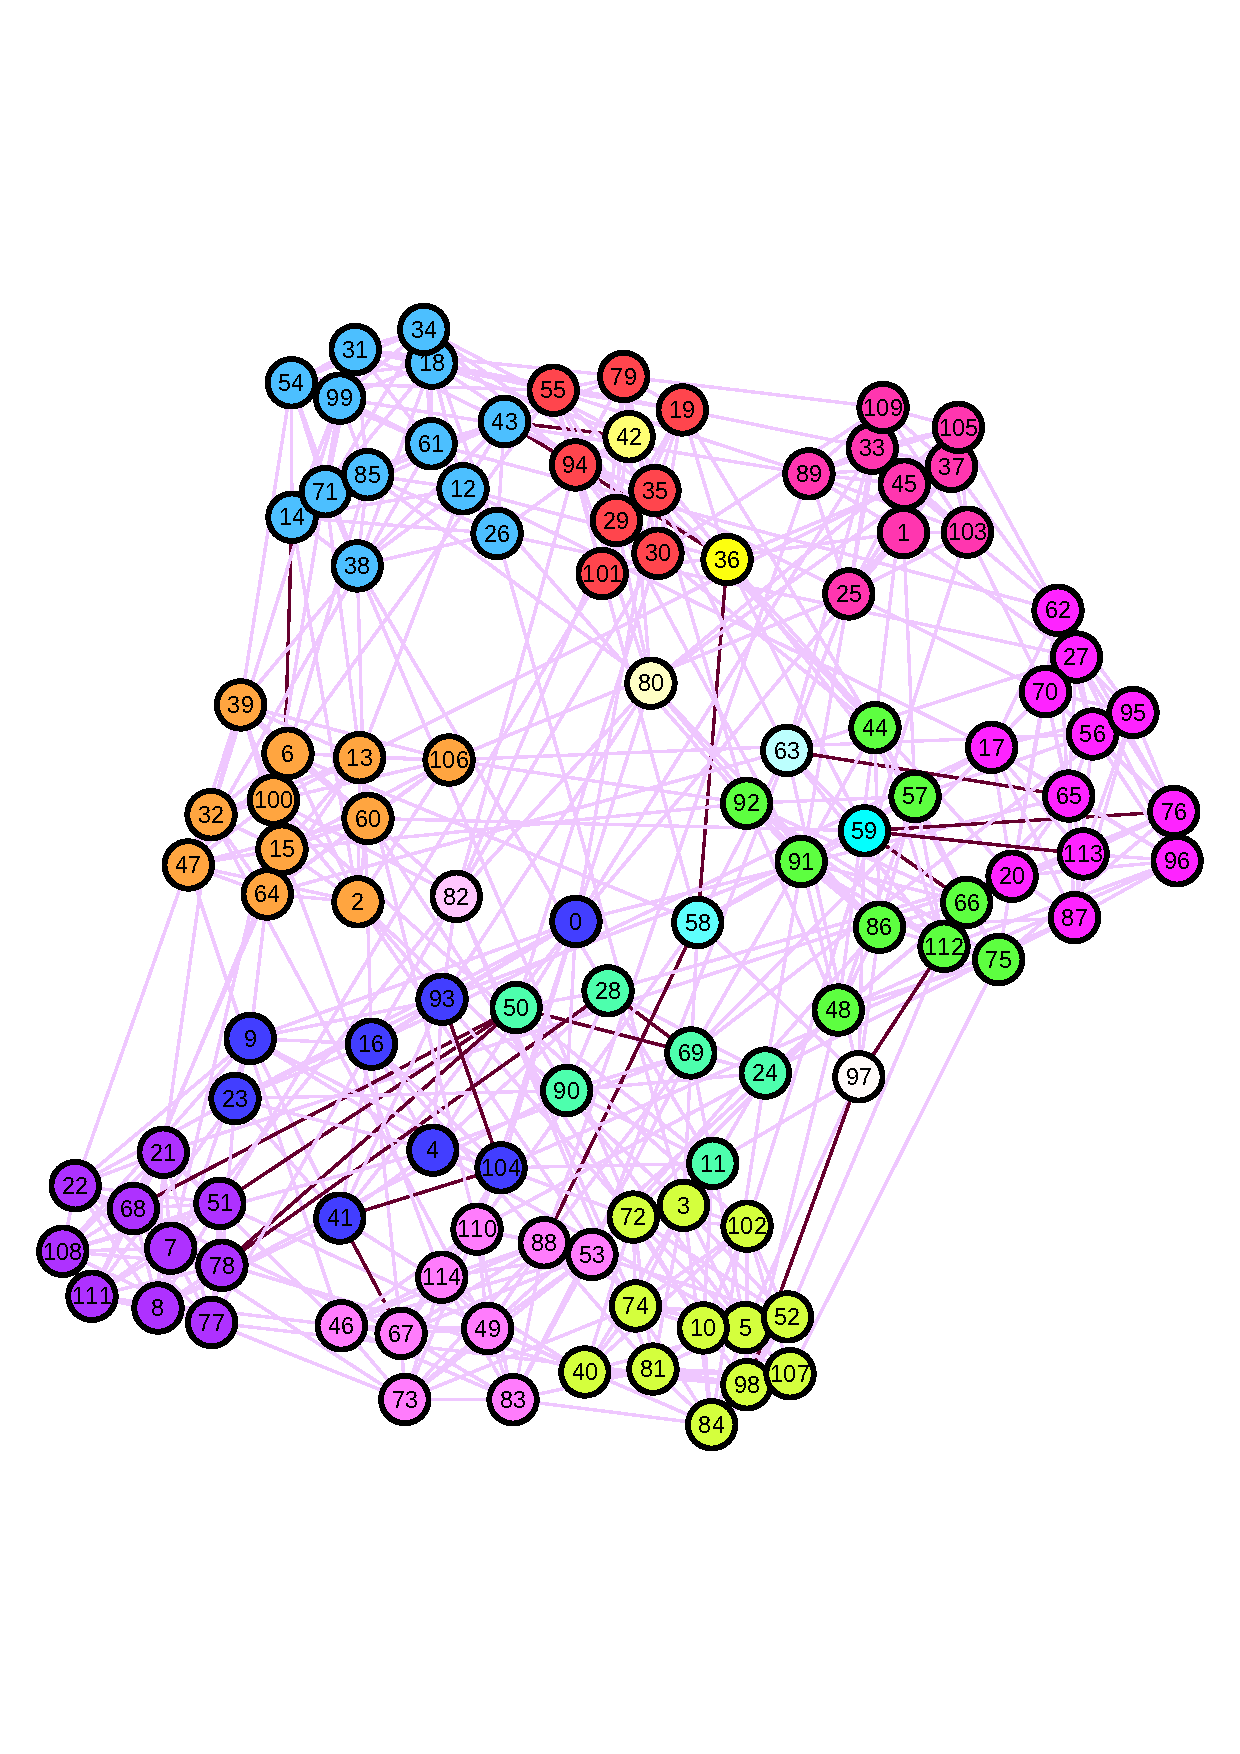
\includegraphics[width=.99\linewidth]{img/chap2/football_neg_edge.pdf}
\caption{}\label{fig:football_groundtruth}
\end{subfigure}
\begin{subfigure}{.3\textwidth}
\centering
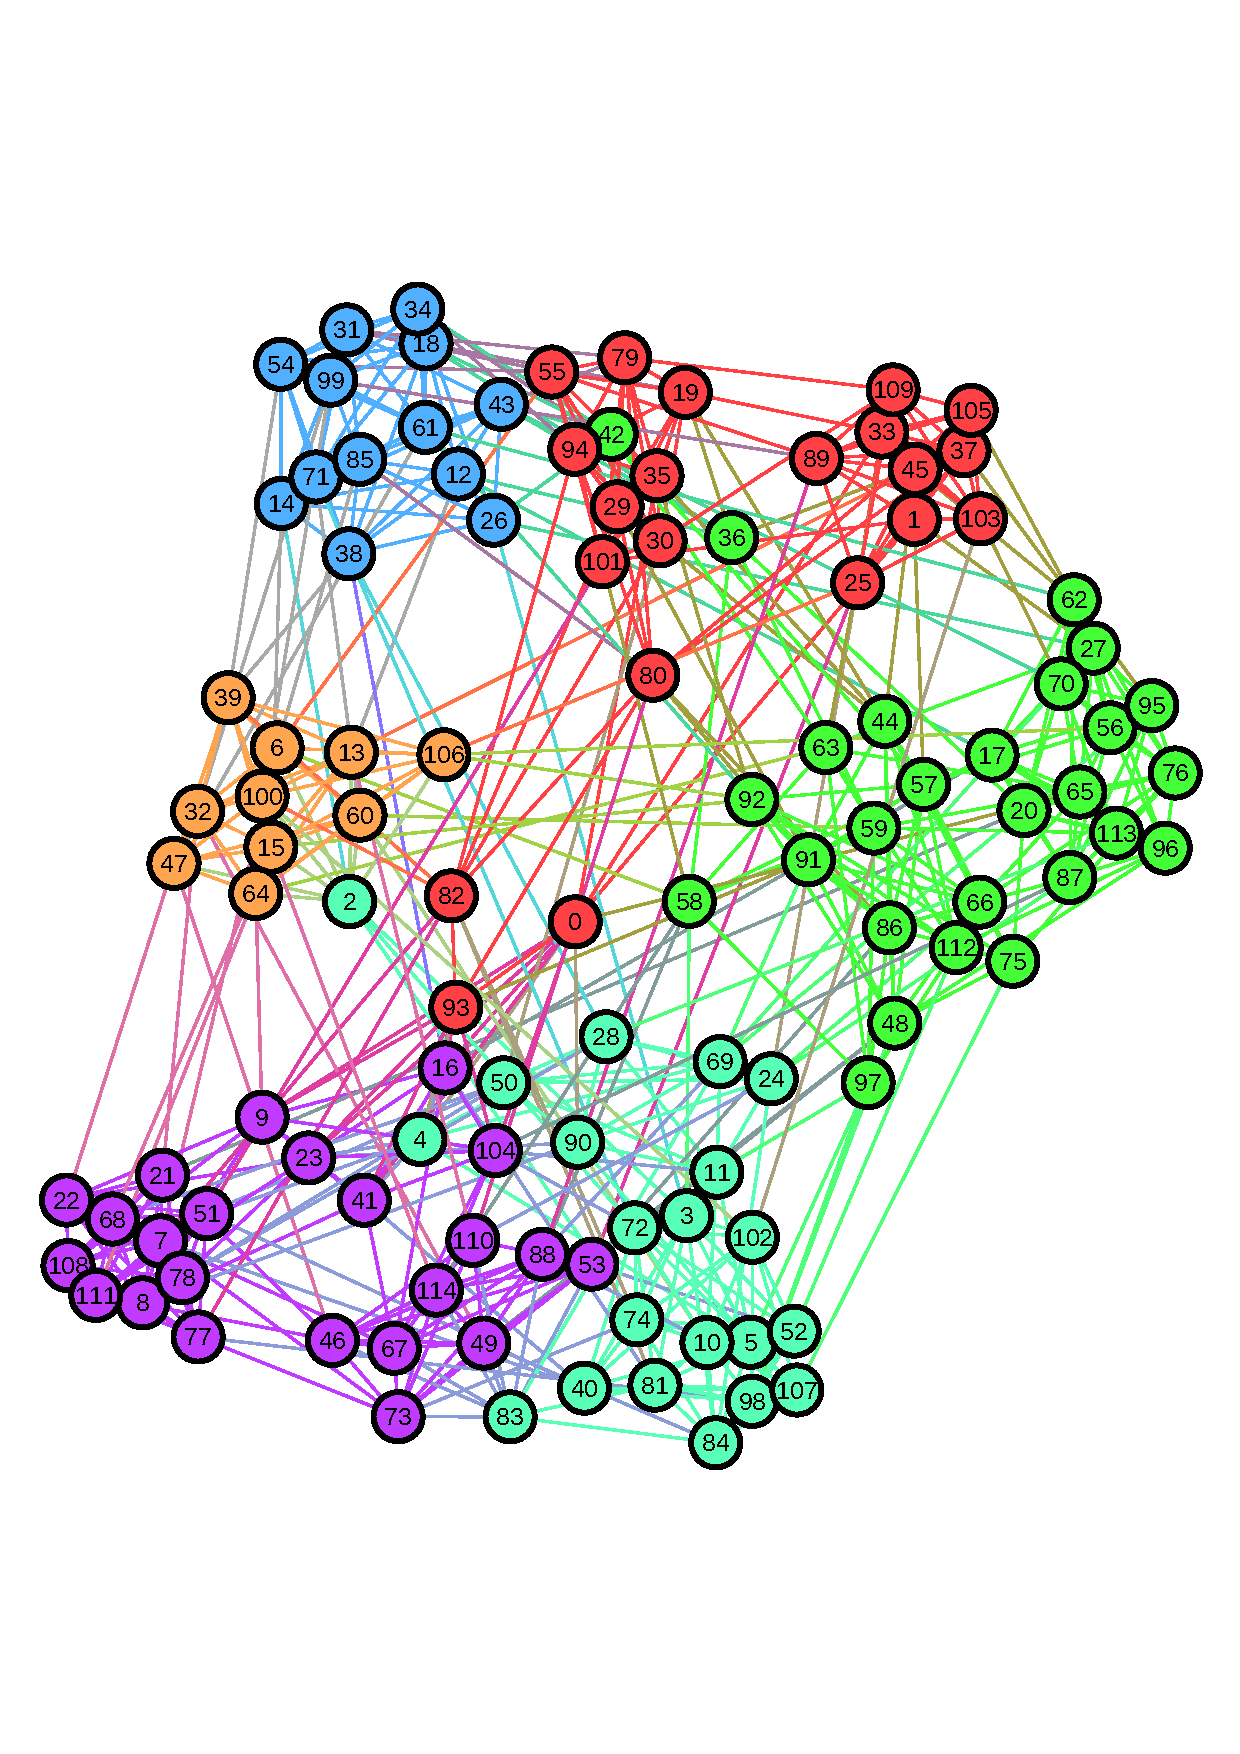
\includegraphics[width=.99\linewidth]{img/chap2/football_orig.pdf}
\caption{}
\label{fig:football_orig}
\end{subfigure}
\begin{subfigure}{.3\textwidth}
\centering
\includegraphics[width=.99\linewidth]{img/chap2/football_better.pdf}
\caption{}
\label{fig:football_better}
\end{subfigure}
\caption{The communities detected by the Fast Greedy algorithm~\cite{clauset2004finding} in the American college football network~\cite{evans2010clique}. Nodes are colored according to communities to which they have been assigned. (a) 19 ground truth communities defined as 11 conferences and 8 independent teams. Edges in black are assigned negative weights by the edge weighting scheme. (b) 6 communities detected on the unweighted graph by the modularity maximization method. (c) 11 communities detected on the weighted graph by the modularity maximization method.}
\label{fig:football_convergence}
\end{figure}
\textbf{American college football network} \label{sec:football}
The American college football network~\cite{evans2010clique} consists of 115 nodes representing college football teams playing in a league with 11 conferences. Two teams are linked if they have played with each other in the year 2000 season. The teams in each of the 11 conferences can be treated as one community because they play with each other often. There are 8 independent teams (not members of any conference), each forming a single community. 19 ground truth communities are shown in Figure~\ref{fig:football_convergence}.a with each color representing a single community. However, only 6 communities are detected by the Fast Greedy algorithm on an unweighted graph as shown in Figure~\ref{fig:football_convergence}.b because some adjacent ground truth communities are joined together.
\begin{table}[!t]
\caption{Metric values characterizing the community structures computed over the original unweighted American college football network but discovered in either the original unweighted graph or the corresponding weighted graph produced by our model.}
\label{table:football}
\centering
\setlength\tabcolsep{2pt}
\begin{tabular}{ |c|c|c|c|c|c|c| }
 \hline
Metric & Graph & FG & LE & LP & RW & ML \\
 \hline
 \multirow{2}{*}{NMI} & Original &0.58528&0.58140&0.76962&0.83833&0.83391\\
 & Weighted & 0.91117&0.85903&0.92635&0.91117&0.87272\\
\hline
 \multirow{2}{*}{ARI} & Original &0.49333&0.49441&0.71749&0.86938&0.85815\\
 & Weighted &0.94723&0.88982&0.91539&0.94723&0.90085\\
 \hline
 \multirow{2}{*}{$Q$} & Original &
 0.56860&0.49326&0.57668&0.60337&0.60503\\
 & Weighted & 0.60140&0.59338&0.57315&0.60140&0.60356\\
 \hline
 \multirow{2}{*}{$Q_{ds}$} & Original &0.15877&0.13661&0.21106&0.23650&0.23626\\
 & Weighted &0.25696&0.23893&0.24025&0.25696&0.24889\\
 \hline
\end{tabular}
\end{table}
The regression model converts the original unweighted graph to a weighted graph where the edges with negative weights are marked in black in Figure~\ref{fig:football_convergence}.a. On the weighted graph, the Fast Greedy algorithm can find 11 league communities, each containing one individual conference, although it allocates the independent teams to some of these league communities. The regression model is trained by sampling the ground truth communities on the artificial SBM network, which is constructed to be similar to the Football network. The training process takes approximately 10 seconds on a machine with a single 2.5GHz CPU.
Table~\ref{table:football} lists the results of the followings approaches: Fast Greedy algorithm~\cite{clauset2004finding} (FG), leading eigenvector method~\cite{newman2006finding} (LE), label propagation algorithm~\cite{raghavan2007near} (LP), community detection based on random walks~\cite{pons2005computing} (RW), multilevel algorithm~\cite{blondel2008fast} (LW) measured by the normalized mutual information (NMI) and adjusted rand index (ARI). As illustrated in Table~\ref{table:football}, in addition to the Fast Greedy modularity maximization algorithm, the state-of-the-art community detection algorithms, including label propagation algorithm by Raghavan et al.~\cite{raghavan2007near}, Newman's leading eigenvector method~\cite{newman2006finding}, the algorithm based on random walks~\cite{pons2005computing} and the multilevel algorithm by Blondel et al.~\cite{blondel2008fast}, also demonstrate improved performance on weighted graphs produced by our method\footnote{In the experiments, the edges with negative weight are removed from the graph because some community detection algorithms are not able to handle negative weights due to the algorithm design or implementation.}. This result additionally supports our claim that properly weighting a graph can lead to an improved quality of community detection.
For a fair comparison, regardless of whether the partition of the graph is determined with or without the edge weights, both the modularity $Q$ and modularity density $Q_{ds}$ are computed over the unweighted graph, i.e., edge weights are all set to 1. Hence, a better $Q$ or $Q_{ds}$ found on the weighted graph indicates the edge weights allow the maximization algorithm to avoid the inferior local optima. The NMI and ARI measures indicate that the communities detected in the weighted graph are generally accurate. However, from the aspect of modularity, for three algorithm, LP, RW and ML, such communities may be evaluated as inferior (as they have slightly lower modularity) than the communities discovered in the original unweighted graph. Consequently, even if the maximum modularity is reached in the original unweighted graph, the resulting communities are still not likely to match the ground truth. In contrast, the modularity density $Q_{ds}$\footnote{Note that the modularity density values are all computed over the original Football network.} of the communities detected in the weighted one is higher than in the original unweighted graphs, which means that it accurately measures the quality of these communities. The proposed edge weighting scheme leads to a higher modularity density $Q_{ds}$ in all cases because the weighted edges allows the greedy algorithm to escape from local maximum of $Q_{ds}$ and get better value of it on the original unweighted graph. 
\begin{figure}[ht!]
\centering
\begin{subfigure}{.45\textwidth}
\centering
\includegraphics[width=.9\linewidth]{img/chap2/comm_distribution_amazon.pdf}
\caption{Amazon}
\label{fig:1}
\end{subfigure} %    <-- % added here
\hfill %% useful if width of each figure is less the .5\textwidth
\begin{subfigure}{.45\textwidth}
\centering
\includegraphics[width=.9\linewidth]{img/chap2/comm_distribution_dblp.pdf}
\caption{DBLP}
\label{fig:2}
\end{subfigure} \\
\begin{subfigure}{.45\textwidth}
\centering
\includegraphics[width=.99\linewidth]{img/chap2/fmeasure.pdf}
\caption{F-measure}
\end{subfigure} %    <-- % added here
\hfill %% useful if width of each figure is less the .5\textwidth
\begin{subfigure}{.45\textwidth}
\centering
\includegraphics[width=.99\linewidth]{img/chap2/execution_time.pdf}
\caption{Efficiency}
\end{subfigure} \\
\caption{Performance improvement of community detection in Amazon and DBLP networks.}
\label{fig:comm_distribution}
\end{figure}
\textbf{Large Networks} We evaluate the performance of our model on two large real networks: Amazon co-purchasing network and DBLP co-authorship network. The Amazon co-purchasing network~\cite{yang2015defining} consists of 334,863 products with two frequently co-purchased products linked by an undirected edge. Each collection of products from the same category forms one ground-truth community. The DBLP collaboration network~\cite{yang2015defining} is the co-authorship network where every node represents a researcher. Two researchers who published at least one paper together are linked. Following others, we assume that individual ground-truth community is defined by the publication venue, e.g., journal or conference. 
The proposed weighting scheme is compared with the wCNM\_1 algorithm~\cite{berry2011tolerating} which computes the weight of an edge using all the triangles and 4-cycles containing it. In our experiments, the wCNM\_1 algorithm iterates only once over updates, because the results in~\cite{berry2011tolerating} show that additional iterations negligibly improve the final results. The regression model which converts the original unweighted graphs to weighted ones is trained by sampling the dynamically constructed artificial SBM networks. In addition, we also test the performance of our model trained by the ground truth communities in the American college football network, as shown in Figure~\ref{fig:comm_distribution}. Perhaps surprisingly, the accuracy of the modularity maximization algorithm on the weighted graph when weights were based on SBM artificial network has improved for the Amazon network by almost 50\% as measured by F-score and even more for the DBLP network. 
The sizes of communities discovered in Amazon and DBLP networks containing more than $3$ nodes are plotted in Figure~\ref{fig:comm_distribution}a-b. In the weighted graph produced by our model for the Amazon network, the distribution of the sizes of the detected communities is close to the distribution of the sizes of ground truth communities for weights based on SBM artificial network but quite different for weights based on the Football network. Since the F-score was similar for those two cases, this result demonstrates the importance of inspecting the distribution of the community sizes. In case of the DBLP network, the improvement of F-score is significant for the weights based on the SBM network, but the distribution of the community sizes is different. We believe that these two results show that presumed ground truth communities in DBLP are not correct, and that smaller communities of researchers co-authoring papers across several venues are the right communities. These results show that our model successfully converts large networks to the weighted ones where the modularity maximization algorithms can perform better than they do on the original unweighted networks.
In general, these large networks can be processed in a few minutes as shown in Figure~\ref{fig:comm_distribution}d. The computation time is divided into two parts: (i) Training: the time spent to infer all the parameters of the regression model; (ii) Weighting: the time needed to compute the weights of every edge in the graph. Both steps include the I/O processing time of loading the network files from disk. The edge topological feature extraction (i.e., weighting) time increases as the number of edges grow, therefore processing of dense graphs can be more time-consuming. Unlike the weighting time, the training time does not change much with the size of the original network. This is because the size of the constructed artificial network is independent of the size of the original input graph. Last but not least, in our experiments, the edge topological feature extraction and edge weight evaluation use a single thread implementation. However, as problems that are easily parallelizable, they can be partitioned into many individual tasks to achieve a better performance.


\section{Conclusions} \label{sec:2.7}
Modularity maximization is one of the state-of-the-art approaches for community detection in complex networks. However, due to the resolution limit problem, it tends to merge small, well-formed communities into a large component to increase the modularity. To deal with the resolution limit problem, we propose two key enhancements to the modularity maximization - one assigning proper weights to edges in the network; the other recursively dividing a graph into subgraphs until the remaining communities are statistically significant. The experimental results show that both approaches significantly improves the quality of the detected communities in the real and synthetic networks.

Besides the contributions on the practical community detection algorithms, we also develop the theoretical results for modularity-based community detection. Specifically, we establish the asymptotic lower and upper bounds of the generalized modularity. The lower bound corresponds to the highest background inter-community edge density in a network, while the upper bound corresponds to the lowest intra-community edge density. This work connects the resolution limit of modularity with random graph theories, which also reveals the ``plateaus" problem that no universal resolution parameter exists to detect all centers. The issue is analogous to finding mountains that are located at different plateaus; using a single altitude either would miss the lower mountains, or would treat the higher peaks as one mountain.

The stochastic block model can produce a wide variety of different network structures, including traditional assortative communities and different from them disassortative structures. In theory, it should be possible to guide the inference algorithm which type of structure is preferred when both types of structures fit the stochastic block model and its degree-corrected variant well for the input network. However, the existence of multiple local optima of the log-likelihood traps the inference algorithms in one of them. We apply a simple yet effective constraint on nodes' internal degree ratio of the degree-corrected stochastic block model. The resulting algorithm reliably finds assortative or disassortative structure as directed by the value of a single regularization parameter. We validated the model experimentally testing its performance on several real and synthetic networks.

Future works include applying more capable models as the nested hypothesis in the significance testing framework and extending the multi-scale community detection algorithm and edge weighting scheme to directed networks.

